\documentclass[10pt,twocolumn,letterpaper]{article}

\usepackage{3dv2016authorkit/latex/3dv}
\usepackage{times}
\usepackage{epsfig}
\usepackage{graphicx}
\usepackage{amsmath}
\usepackage{amssymb}

% Include other packages here, before hyperref.
%\usepackage{multicol}
\usepackage{url}

% If you comment hyperref and then uncomment it, you should delete
% egpaper.aux before re-running latex.  (Or just hit 'q' on the first latex
% run, let it finish, and you should be clear).
%\usepackage[pagebackref=true,breaklinks=true,letterpaper=true,colorlinks,bookmarks=false]{hyperref}

%\threedvfinalcopy % *** Uncomment this line for the final submission

\def\threedvPaperID{4} % *** Enter the 3DV Paper ID here
\def\httilde{\mbox{\tt\raisebox{-.5ex}{\symbol{126}}}}

% Pages are numbered in submission mode, and unnumbered in camera-ready
\ifthreedvfinal\pagestyle{empty}\fi
\setcounter{page}{4321}
\begin{document}

%%%%%%%%% TITLE
\title{A Large-Scale 3D Object Recognition dataset}

\author{Thomas S{\o}lund\\
Danish Technological Institute\\
DK-5230 Odense M, Denmark\\
{\tt\small thso@dti.dk}
%For a paper whose authors are all at the same institution,
% omit the following lines up until the closing ``}''.
% Additional authors and addresses can be added with ``\and'',
% just like the second author.
% To save space, use either the email address or home page, not both
\and
Anders Glent Buch, Norbert Kr\"u{}ger\\
M\ae{}rsk Mc-Kinney M\o{}ller Institute,\\
University of Southern Denmark,\\
DK-5230 Odense, Denmark \\
{\tt\small anbu,norbert@mmmi.sdu.dk}
\and
Henrik Aan\ae s\\ %Knut Conradsen, 
Department of Applied Mathematics\\ and Computer Science,\\ 
Technical University of Denmark\\
DK-2800 Kgs. Lyngby, Denmark\\
{\tt\small aanes@dtu.dk} %knco,
}

\maketitle
%\thispagestyle{empty}

%%%%%%%%% ABSTRACT
\begin{abstract}
  This is dummy text. This is dummy text. This is dummy text. This is dummy text. This is dummy text. This is dummy text. This is dummy text. This is dummy text. This is dummy text. This is dummy text. This is dummy text. This is dummy text. This is dummy text. This is dummy text. This is dummy text. This is dummy text. This is dummy text. This is dummy text. This is dummy text.This is dummy text. This is dummy text. This is dummy text. This is dummy text. This is dummy text. This is dummy text. This is dummy text. This is dummy text. This is dummy text. To be written...........
\end{abstract}

%%%%%%%%% BODY TEXT

%%%%%%%%%%Page limits = 8 exclusive references
%Intro and related work -> 2.5 page
%Experiantal design -> 1 page
%Benchmark -> 1 page
%Evaluation/results -> 3 pages
% conclusion/discussion -> 1/2 page
\section{Introduction} %Hvad, hvorfor, hvordan
The ability to recognise objects in range images is a fundamental research area in computer vision with many different application areas. With continually introduction of new affordable 3D sensors for different applications, the ability to localize and recognize rigid and no rigid objects are a attractive and unavoidable technology in the future. Applications areas such as robotic assembly, bin-picking, mobile manipulation, biometric analysis, tracking and intelligent surveillance all benefits from 3D data for recognizing and localizing objects. Mainly, because the third dimension are explicit given and not inferred as known from 2D object pose estimation. In the last decades a huge effort in 2D object recognition and classification has been going on, where methods have been evaluated on large-scale dataset like the PASCAL Visual Object Challenge (VOC) \cite{Everingham2014} and ImageNet \cite{Imagenet2009}. The ability to evaluate algorithms with a large-scale dataset has proven valuable in the future algorithm development after the release of the PASCAL VOC and ImageNet datasets \cite{Everingham2014}.
\begin{figure}[t]
\centering
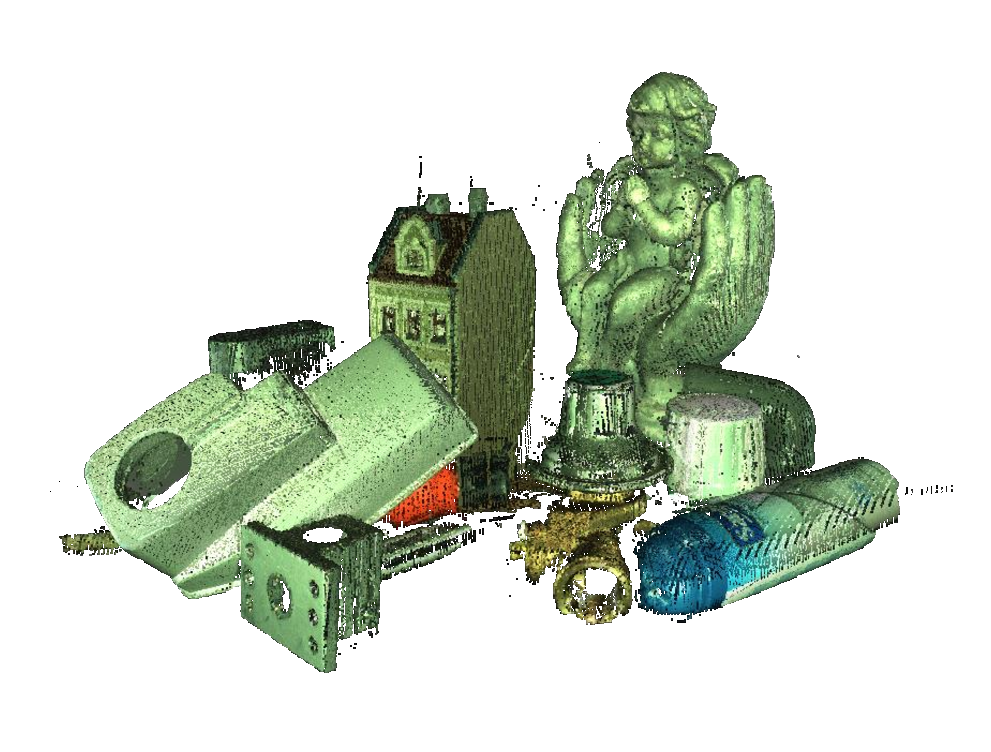
\includegraphics[width=0.8\linewidth, height= 0.8\linewidth, keepaspectratio]{img/scenes/scene_000.pdf}
\caption{Example of a scene}
\label{fig:scene}
\end{figure}
In 3D object recognition and pose estimation there still is a need for a large-scale dataset that consistes of 3D querie models $Q_n$, 3D target scenes $S_t$ and ground truth poses $T_{gt}$ for each object in each scene, in order to be able to evaluate 3D object recognition algorithms better. Until today 3D object recognition has been evaluated at up to eight smaller datasets \cite{Guo2015}, include in the UWA \cite{Mian2006},\cite{Mian2010}, Queens \cite{Taati2007},\cite{Taati2007} and Bologna \cite{Salti2014},\cite{Tombari2010} dataset. Other, smaller dataset like the Vienna Kinect\cite{Aldoma2012}, TUM \cite{Rodola2013}, TUM-LineMod\cite{Hinterstoisser2012}, BigBird\cite{BigBIRD} and RGB-D dataset version 1 \& 2\cite{Lai2011}, \cite{Lai2014} have been proposed. Common for all dataset are that the amount of scenes and/or models are limited.\\
%\begin{multicols}{3}
\begin{table*}[ht]
\label{tab:datasets}
\centering % Center table
         \begin{tabular}{p{4.2cm} p{0.3cm} p{1.2cm} p{1.5cm} p{1.55cm} p{0.3cm} p{0.3cm} p{0.3cm} p{0.3cm} p{0.3cm} p{0.3cm} p{0.3cm} p{0.3cm} p{0.3cm} p{0.3cm}}
                  %%  & \multicolumn{2}{c}{Data Size} & \multicolumn{4}{c}{Models} & \multicolumn{2}{c}{Scene} & \multicolumn{5}{c}{Ground truth} & he \\
                  %%  \hline
             & {$M_q$} & {$S_t$} &  Sensor & {$M_q$} in {$S_t$} & \rotatebox{90}{$M_q$ normals} & \rotatebox{90}{$M_q$ color } & \rotatebox{90}{$M_q$ mesh } & \rotatebox{90}{$S_t$ normals } & \rotatebox{90}{$S_t$ color } & \rotatebox{90}{$S_t$ mesh} & \rotatebox{90}{Full 6D pose} & \rotatebox{90}{Occlusion} & \rotatebox{90}{Clutter} & \rotatebox{90}{[R]/[S]}\\
            \hline
            \hline
             UWA \cite{Mian2006}, \cite{Mian2010}  & 5 & 50 & LIDAR & (5)/(5) & \checkmark & \% & \checkmark & \checkmark & \%  & \checkmark & \checkmark  & \checkmark & \% & R\\
             \hline
             Queens Lidar  \cite{Taati2011}, \cite{Taati2007}  & 5 & 80 & LIDAR & (1-5)/(1-5) & \checkmark & \% & \checkmark & \% & \%  & 0 & \checkmark & \% & \% & R\\
             \hline
             Queens Stereo  \cite{Taati2011}, \cite{Taati2007}  & 5 & 100 & Stereo & (3)/(3)   & \checkmark & \% & \checkmark & \% & \%  & 0 & \checkmark & \% & \% & R\\
             \hline
             Bologna 1\&2 \cite{Salti2014}, \cite{Tombari2010} & 6 & 45 & - & (3-5)/(3-5) & \checkmark & \% & \checkmark & \checkmark & \% & \checkmark & \checkmark & \% & \% & S \\
			 \hline              
             Bologna 3 \cite{Salti2014}, \cite{Tombari2010} & 8 & 15 & Spacetime & (2)/(5-6) & \checkmark & \checkmark & \% & \checkmark & \checkmark & \checkmark & \checkmark & \% & \% & R\\
             \hline
             Bologna 4 \cite{Salti2014}, \cite{Tombari2010} & 8 & 16 & Spacetime & (2)/(6) & \checkmark & \checkmark & \% & \checkmark & \checkmark & \checkmark & \checkmark & \% & \% & R\\
             \hline
             Bologna 5 \cite{Salti2014}, \cite{Tombari2010} & 6 & 16 & Kinect V1 & (2-4)/(5-9) & \checkmark & \checkmark & \% & \checkmark & \checkmark & \checkmark & \checkmark & \% & \% & R \\
             \hline
             Vienna Kinect \cite{Aldoma2012} & 35 & 50 & Kinect V1 & 0 & \checkmark & \% & \checkmark & \% & \checkmark & 0 & \checkmark & \% & \% & R\\
             \hline
             RGB-D Scenes V1 \cite{Lai2011}, \cite{Lai2012} & 5 & 8 videos & Kinect V1 & (0)/ & \% & \% & \%  & \% & \checkmark  & \% & \% & \% & \% & R\\
			 \hline             
             RGB-D Scenes V2 \cite{Lai2014} & 9 & 14 & Kinect V1 & (0)/ & \% & \% & \% & \% & \checkmark & \% & \% & \% & \% & R\\
             \hline
             T{\"U}M \cite{Rodola2013} & 20 & 150 & - & (3-5)/(3-5) & \checkmark  & \%  & \checkmark  & \checkmark & \% & \checkmark & \checkmark & \checkmark & \checkmark & S\\
             \hline
             Willow \cite{Willow} & 35 & 177 & Kinect V1 & 0 & \checkmark  & \checkmark  & \checkmark  & \% & \checkmark & 0 & \% & \% & \% & R\\
             \hline
            % B3DO \cite{Janoch2011}  & 0 & 849 & kinect & 0 & \%  & \%  & \%  & \% & \checkmark & \% & \% & \% & R\\
            % \hline
             ECCV12 \cite{Aldoma2012}  & 35 & 50 & Kinect V1 & (3-7)/(3-7) & \%  & \checkmark  & \checkmark  & \% & \% & \% & \checkmark & \% & \% & R\\
             \hline
              Alicante \cite{Garcia-Garcia2016}  & 30 & 50 & Kinect V2 & (0)/(0) & \%  & \checkmark  & \checkmark  & \% & \% & 0 & \checkmark & \% & \% & R\\
             \hline
             \hline
             \textbf{Our SL dataset}  & \textbf{50} & \textbf{3300} & SL & (10)/(10) & \checkmark  & \checkmark  & \checkmark  & \checkmark & \checkmark & \checkmark & \checkmark  & \checkmark & \checkmark & R\\
             \hline
             \textbf{Our Kinect dataset}  & \textbf{50} & \textbf{3300} & Kinect V2 & (10)/(10) & \checkmark  & \checkmark  & \checkmark  & \checkmark & \checkmark & \checkmark & \checkmark  & \checkmark & \checkmark & R\\       
             \hline 
        \end{tabular}
%        \captionof{table}{Existing datasets for 3D object recognition and pose estimation}% Add 'table' caption
        \label{dataset_overview}
 
\caption{Comparison of existing datasets for 3D object recognition with the presented datasets. {$M_q$} is the amount of different models in the dataset and {$S_t$} is the amount of scenes.[R]/[S] indicates whether the dataset is synthetic or acquired in real world. }
\end{table*}
%\end{multicols}
In this work we present a new large-scale dataset consisting of 50 objects and 3300 scenes. The new dataset is recorded systematically in an environment without ambient light and with controlled illumination. The system includes a industrial robot in a dark chamber, a high precision structured light scanner and a Kinect V2 sensor, which records data from 11 different view points. Each scene consists of 10 objects automatic taken with the two different sensors, which results in a dataset with around 66000 unique object poses. With 11 different views of the same scene our dataset is especially suited for studying the effect of view point changes in 3D object recognition. Our 50 object models are scanned in a similar dark chamber with a high precision structured scanner and a rotation table. With this setup we are able to scan objects with an accuracy down to XX microns. We use the dataset to evaluate state of the art local shape features in a 3D object recognition pipeline. In Table \ref{tab:datasets} a summery of the features of ours and state of the art dataset are presented.\\
Why do the 3D Object recognition community needs another dataset? Current proposed dataset is limited in the number of objects/scenes and the objects included in the datasets are mostly geometrical ideal objects. With geometrical ideal objects we refers to mostly concave objects that are rich of geometrical features like the UWA-chef model \cite{Mian2006},\cite{Mian2010}, the bologna-Armadillo \cite{Salti2014},\cite{Tombari2010} and the Queens-BigBird \cite{Taati2007},\cite{Taati2007}. With our dataset we introduce not only ideal concave objects, but flat, cylindrical, feature-rich and feature-poor concave and convex objects. Our objects are a combination of lab-objects and industrial objects which are selected from companies that wants to pick these objects from boxes or bins with a robot.\\
This paper is structured as follows: In Section \ref{sec:related_work} related datasets and local feature descriptors are presented. Section \ref{sec:exp_design} details our experimental design followed by Section \ref{sec:benchmark} which presents our benchmarking methodology. In Section \ref{sec:evaluation} the results are given followed by a discussion and conclusion in Section \ref{sec:conclusion}. 
%-------------------------------------------------------------------------
\section{Related work} \label{sec:related_work}
%We are not considering learning approaches
\textbf{3D Object Recognition datasets:}\\
The last 10 years a few 3D object recognition datasets have been published. Mainly in conjunction with algorithms for local feature description \cite{Mian2006},\cite{Taati2007},\cite{Taati2011},\cite{Tombari2010},\cite{Salti2014}, correspondence matching and rejection \cite{Rodola2013}, pose hypothesis verification \cite{Aldoma2012} and 3D keypoint detection \cite{Mian2010}. Common for all existing dataset are the limited number of 3D object models and scenes. A comparison of the different datasets are presented in Table \ref{tab:datasets}. The most common used datasets are the UWA  \cite{Mian2006}, \cite{Mian2010}, Queens \cite{Taati2007},\cite{Taati2011} and the Bologna \cite{Salti2014}, \cite{Tombari2010}. These datasets are widely used in performance evaluations of  local feature descriptors \cite{Guo2015}, \cite{Buch2016}, keypoint detectors \cite{Salti2011} and surveys \cite{Guo2014}, \cite{FilipeAlexandre2014}. The main problem of all the datasets are; size, variety of objects and occlusion/clutter estimates. The recent comparison studies \cite{Guo2015}, \cite{Buch2016} revival that the data for evaluation are not good enough to scientific distinguish results. The studies exactly showed that one local feature descriptor preformed very good for one dataset but fail in other datasets. The reason could be twofold; the local feature descriptors are not generalizing well and/or the evaluation data is too limited. This work tries to answer this question.\\ 

\textbf{Local feature descriptors:}\\
{\color{red} AGB will you write this. Length around 1 colum}
During the last three decade, a vast number of different 3D local feature descriptors have been proposed including SPLASH \cite{Stein1992}, Spin Image (SI) \cite{Johnson1999}, 3D Shape Contex (3DSC) \cite{Frome2004}, LSP \cite{ChenBhanu2004}, 3D Tensor \cite{Mian2006}, THRIFT \cite{Flint2007}, MESH-HOG \cite{Zaharescu2009}, ISS \cite{Zhong2009}, Unique shape context (USC) \cite{usc2010}, Point Feature Histogram (PFH)\cite{Rusu2008}, Fast Point Feature Histogram (FPFH) \cite{Fpfh2009}, SHOT \cite{Tombari2010}, ROPS \cite{Guo2013}, ECSAD \cite{Ecsad2015}, Tri-Spin-Image (TriSI)\cite{Guo2015}. The descriptors find usages in applications such as 3D object categorization, recognition, retrial, analysis, registration and reconstruction among others. Designing descriptors which are distinctive and robust to occlusion and noise are still and ongoing research topic. Recent studies has shown that the proposed features are not generalizing well over many types of geometry classes, \cite{Guo2015},\cite{Buch2016}. The studies proved one of the main issue in 3D object recognition today, namely the fact that there exist no local shape feature that describes the geometry well in many different object classes, e.g. flat, rotational symmetrical and geometrical feature rich objects. What feature(s) to use are still dependant of the object geometry. These studies poses a relevant research question, are the local feature descriptors not descriptiveness enough to generalize over different object classes or are the evaluation data to limited? The evaluation dataset there are used for the evaluation in general and in \cite{Guo2015},\cite{Buch2016}, consists mainly of objects with many descriptive and distinctive geometrical features. In this work we try to answer this fundamental question by creating the data foundation to evaluate the performance of each local feature descriptors by applying statistic. 

Local feature descriptor aims at computing a distinctive and robust N-dimensional feature vector around a point, by considering the k-neighbour points in euclidean space. The radius of the K-Nearest Neighbour search (KNN), the support radius is often one of the critical parameters in the pipeline. Local feature descriptors are often split into tow different categories, spatial and geometrical histograms \cite{Guo2015}. Global feature descriptors, typical computes a descriptors by considering the spatial and/or geometrical relations between two or more local feature descriptors on a 3D geometry.   

Local shape features can be split into two different categories, spatial and geometrical histograms \cite{Guo2015}. 
Early work by Stein and Medioni \cite{Stein1992} used a combination of edges and small surfaces patches for 3D matching in range images. Later Johnson  and Albert introduced Spin Images \cite{Johnson1999} 

Spin Images \cite{Johnson1999}\\
Froome \etal \cite{Frome2004} presented a local descriptor 3D shape context.
%USC \cite{usc2010}\\

%PFH \cite{Rusu2008}
%FPFH \cite{Fpfh2009}\\
%ECSAD \cite{Ecsad2015}\\
%ROPS \cite{Guo2013}\\
%SHOT \cite{Salti2014}\\
%NDHIST\\
%PPF \cite{Drost2010}\\
%SHOT \cite{Tombari2010}\\

Recently, a couple of benchmarks of local feature descriptors has been presented. Guo \etal \cite{Guo2015} presented a comprehensive comparison of most common local feature descriptors. The 
Feature Fusion \cite{Buch2016}\\
Feature comparision Yulan et.al. \cite{Guo2015}

%and pose estimation \cite{Viksten09}, \cite{Hinterstoisser2012}, this kind of scientific validations of results still lacks in 3D object recognition. 
%2D object recognition is well studied lacking with 3D. Keypoint comparison Aan{\ae}s et.al. \cite{Aanaes2011}

%We study the performance of the top six local shape features and one global descriptor 
%Limitations in current dataset and algorithms. Feature rich objects not flat or cylindrical objects

%The UWA dataset by Mian et.al. \cite{Mian2006}, \cite{Mian2010} is one of the best known datasets for 3D pose estimation algorithm evaluation. The dataset is composed of four full object models and 50 real scenes captures with a laser scanner which containing incomplete instances of the objects. Each scene contains three or four object models which results in much clutter and occlusion. The amount of occlusion and clutter in each scene is not provided. The four object models are generated with a multi-view registration algorithm. Each object model contain more than 100000 mesh vertices and posses good and distinctive shape features with non-uniform surfaces and ambiguities. The object models and scenes has pre-estimated normals and no color/texture. The dataset contains full 6D ground truth poses for each object as the only evaluation data type.

%The Queens Lidar dataset \cite{Taati2011}, \cite{Taati2007} is constructed like the UWA dataset with a laser scanner and consists of five object models and 80 real scenes take from one viewpoint. Like the UWA dataset, the Queens Lidar dataset contains no color information but the scenes has larger variation compared to the UWA dataset with one to five object models present in the scenes. The five object models has pre-estimated normals but is only provided as a point representation. The dataset contains full 6D ground truth poses for each object as the only evaluation data.

%The Queens Stereo dataset \cite{Taati2011}, \cite{Taati2007} contains five full object models and 100 real scenes created with a stereo camera and standard stereo reconstruction. The dataset is taken from one viewpoint. Each scene contains three object models with no color, normal, occlusion or clutter information available. Like the Queens Lidar dataset the object models is represented with points and no vertices. The dataset contains full 6D ground truth poses for each object as the only evaluation data.

%The Bologna 1 \& 2 dataset \cite{Salti2014}, \cite{Tombari2010} contains six full object models and 45 synthetic scenes. All scenes is construct a synthetic scenes with models from the Stanford 3D Scanning Repository. Each 45 scenes are created by applying a random transformation to a random subset of object model and store the scene. The difference between the Bologna 1 and Bologna 2 dataset are that Bologna 2 is re-sampled 1/8 of the original point density. The fact that it is a synthetic dataset results in 100 percent accurate 6D ground truth data.
%The Bologna 3 dataset \cite{Salti2014}, \cite{Tombari2010} contains eight models and 15 scenes. Each scenes are acquired with spacetime stereo technique and contains both color and surface normal information. Each scene contains two object models and additional objects to create clutter and occlusion. The eight models are single view object templates with color and estimated normals in mesh representation. The dataset contains full 6D pose estimates as ground truth. Their exist no data on occlusion and clutter estimates.
%The Bologna 4 dataset \cite{Salti2014}, \cite{Tombari2010} contains eight models and 16 scenes. As Bologna 3, this dataset is acquired with spacetime stereo techniques and containing color and normal data for both the object models and the scenes. The dataset includes object models with highly similar shapes but different textures. Each scene contains two object models and additional objects to create clutter and occlusion. The eight models are single view object templates with color and estimated normals in mesh representation. The dataset contains full 6D pose estimates as ground truth. Their exist no data on occlusion and clutter estimates.
%The Bologna 5 dataset \cite{Salti2014}, \cite{Tombari2010} contains six object models and 16 scenes. The dataset is acquired with a Microsoft Kinect sensor and includes color and normal information for both the object models and scenes. The provided object models is a set of object templates taken from different views. With a proper mesh registration algorithm a full object model can be created. The dataset contains full 6D pose estimates as ground truth. Their exist no data on occlusion and clutter estimates.
%The Vienna Kinect dataset \cite{Aldoma2012} contains 35 full object models and 50 scenes. Each scene is acquired with a Microsoft Kinect sensor and includes color information but no pre-estimated normals. All scenes is table top scenes with limited occlusion and clutter. The object models in each scene is distThe 35 object models are full represented mesh models without color but includes pre-estimated normals. 
%The dataset contains full 6D pose estimates as ground truth. Their exist no data on occlusion and clutter estimates.
%TUM dataset \cite{Rodola2013}\\
%RGB-D Dataset V1 \cite{Lai2011}, \cite{Lai2012}\\ 
%RGB-D Dataset V2 \cite{Lai2014}\\ 
%------------------------------------------------------------------------
\section{Experimental design} \label{sec:exp_design}
%Describe the object scanning process
\subsection{Object model scanning}
Our object models are scanned with a high precision structured light setup consisting of two industrial cameras (Point Grey Research GS3-U3-91S6C-C) and
a high resolution DLP projector (LG PF80G) mounted on a rigid aluminium frame. In addition, a high precision turntable (Newmark Systems RT-5) is used in order to provide automatic rotation of the object. Each of the 50 objects are incremental scanned with a rotation of 20 degrees. All individual scan views are reconstructed by the Line shifting algorithm \cite{Guehring2000} which results in accurate and dense point cloud of the objects. Eleven temporal binary gray code patterns are projected followed by eight line shifting patterns. The point resolution of the scanner is XX. Once a single view of the model are scanned, noisy outliers of the measurement are manual removed and surface normals are estimated to ensure consistent normals. All 18 views are registered with Iterative Closest Point (ICP) and the object frame are computed by principal component analysis.
All models are sampled with a Poisson disk sampling algorithm and triangulated with the poisson reconstruction algorithm \cite{Kazhdan2006} with an octree depth=14, Solver divide = x and xx = xx. We use the PCL implementation \cite{RusuCousins2011}. All models are provided as coloured point clouds and triangular meshes, all in the $.ply$ format, see Figure \ref{fig:objects}. Note that the modelling setup is not radiometrical calibrated.
\begin{figure}[ht]
\centering
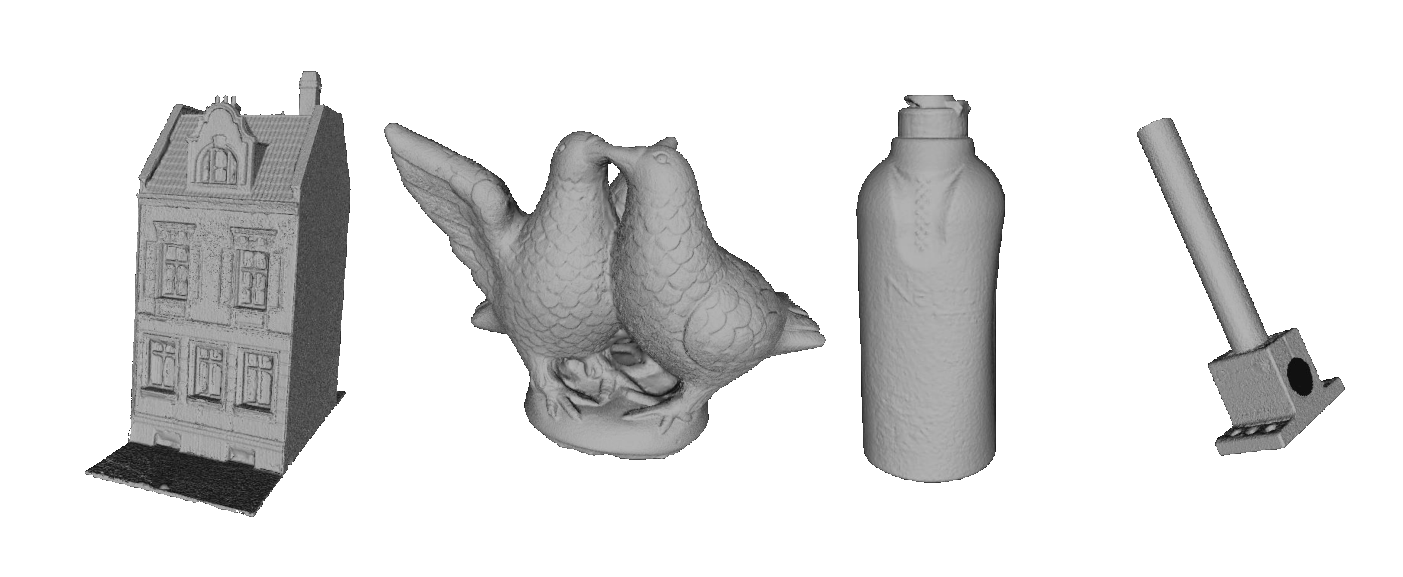
\includegraphics[width=1.0\linewidth, height= 1.0\linewidth, keepaspectratio]{img/objects/objects.pdf}
\caption{Four of the fifty scanned and triangulated object models}
\label{fig:objects}
\end{figure}
%Describe setup for scene aqusition
\subsection{Scene scanning} 
For the data collection we use the robot depicted at Figure \ref{fig:robot}. The robot is equipped with two PointGray Grasshopper3 GS3-U391S6C-C USB3 color cameras with resolution of 9.1 Mp, a Wintech Pro4500 projector with a resolution of 1140x912 pixels and a Kinect One sensor. The sensor cluster is mounted in the robot tool. The sensor modalities are selected by two reasons. First, the structured light system (SL) ensure a high precision that is XX times better than the Kinect thus we are able to provide accurate ground truth pose data for each object in the scene down to a precision of xx mm. Second, Time-of-Flight sensors like the Kinect One sensor are popular sensors in many research areas such as robotic manipulation, 3D semantic mapping, people detection and consumer products thus we wanted to support the future development of 3D object recognition systems and algorithms by including the sensor in the dataset. 
\begin{figure}[ht]
\centering
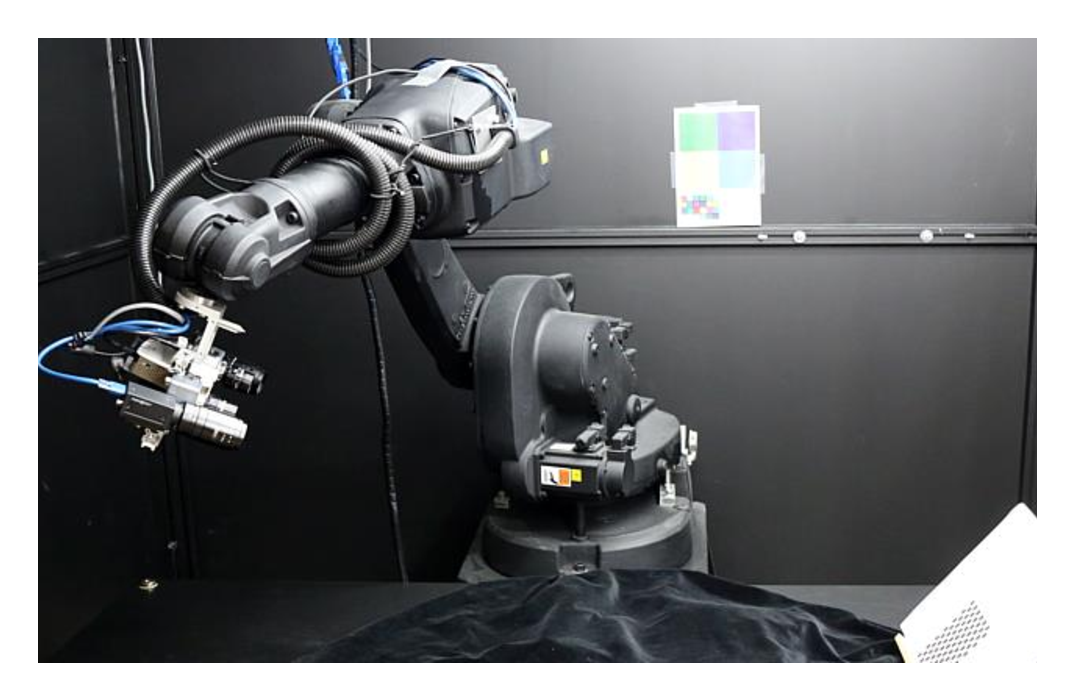
\includegraphics[width=1.0\linewidth, height= 0.7\linewidth]{Robot.pdf}
\caption{Scan of the full scene with view frames}
\label{fig:robot}
\end{figure}
The Robot setup is constructed as a radiometric "dead" which gives a scene representation with zero ambient light. All the scene illumination is controlled in the recording process. The sensor cluster is calibrated with a automatic calibration procedure which includes a stereo calibration of the SL sensor using \verb|OpenCV|\footnote{\url{http://opencv.org/}} and a intrinsic calibration of the Kinect using the \verb|iai_kinect2|\footnote{\url{https://github.com/code-iai/iai_kinect2}} software package. The Kinect calibration ensure a proper registration of the RGB values at each 3D point. An automatic hand eye calibration \cite{DornaikaHoraud1998} is conducted in order to align the Kinect and the SL scans in the world frame. The world frame is the robot base frame.
%Describe recording procedure
Each scene are scanned from 11 different views with both the structured line scanner (SL) and the Kinect such that each physical scene results in 11 SL and 11 Kinect scenes, 22 scenes in total. During the SL scanning process the chamber is completlty dark in order to increase the signal-to-noise ration of the scan. When the Kinect scene are depicted a two diffuse light projectors are automatical turned on to depict the kinect colors. The level of diffuse scene ligth are empirical dertermined such that the kinect RGB camera not oversaturating.  The structured light scans are reconstructed with the Line shifting algorithm \cite{Guehring2000} with ten temporal pattern levels. The views are distributed equally on a quarter sphere around the scene, such that each scene is depicted from - 90 to 90 degrees horizontally and 0 to 45 degree vertically. In order to reproduce the results we store raw Portable Network Graphics images in full resolution (9.1 MP). De-bayering, white balance, image rectification, pattern decoding and point cloud reconstruction are a off line process.   

%Meshing of the scenes + normal estimation

%A Note on ground truth
\subsection{Ground Truth 6D pose}
For each of the ~3300 scenes the 6D ground truth pose, occlusion and clutter estimates for each object are provided. We estimate the occlusion from Equation \ref{eq:occlusion} and clutter from Equation \ref{eq:clutter} by counting the number of points at the object model which squared euclidean distance to a scene point is less than two times the resolution. Both the object model and the scene are sampled to ensure equal point distance.
\begin{equation}
Occlusion = 1 - \frac{visible object points}{total object points} 
\label{eq:occlusion}
\end{equation}
\begin{equation}
Clutter = 1 - \frac{visible object points}{total scene points}
\label{eq:clutter}
\end{equation}
Accurate ground true poses are ensure by registration of the individual SL scans into one full scene model in world frame which covers the geometric structures of all the models in the particular scene, see Figure \ref{fig:scene}. The hand/eye calibration procedure computes the transformation from each sensor frame to the robot flange such that every transformation is known in the system. With all transformation known, it is trivial to align the kinect scans with full SL scene by applying the transformation $T_{kinect2SL}$ followed by fine ICP registration $T_{ICP}$ on the full resolution SL scene. 
All ~300 combined scenes are manual annotated by selecting four identical points for each model and the scene followed by an estimation of the rigid transform. An iterative ICP, which incremental decrease the max allowed correspondence euclidean distance on the full resolution cloud ensures the ground truth pose. The individual ground truth poses in each sensor view $T{s_n}$ are generate by transforming ground truth pose from the world frame $T_{w}$ to each of the individual sensor frames $T{s_n}$ by applying the equation $T^{w}_{s_n} = $. This methodology guarantees accurate pose in $T{s_n}$ independent of the amount of occlusion. Even in views with limited number of scene point of an object the ground truth pose is accurate. Moreover, we align each Kinect scans in $T{s_n}$ to the SL scan by applying the transform $T=$ which gives an accurate ground truth pose for the noisy Kinect data based on dense and accurate SL data. 

%We provide 6D ground truth poses with RMS error for the final ICP registration. In this way we can guarantee that the overall accuracy of all ground truth poses is within xx mm. 
%Combine the 11 views. The different scans are then aligned with respect to scan number zero by applying
%These view points ensure a good coverage of the scene and provide the needed geometric structure of each object to reliable compute ground truth. 
%alignment two frame 0. alignment of kinect scene and transformation back to the sensor frame.

%-------------------------------------------------------------------------
\section{Benchmark}\label{sec:benchmark}
This section outlines the experimental protocol defined to evaluate of the dataset. The protocol are inspired by the one used by Salti \etal \cite{Salti2014}. The evaluation is divide into two parts; feature matching and recognition. The selected local feature descriptors for our evaluation includes; Spin Image (SI) \cite{Johnson1999}, 3DSC \cite{Frome2004}, PFH \cite{Rusu2008}, FPFH \cite{Fpfh2009}, USC \cite{usc2010}, SHOT \cite{Tombari2010}, ROPS \cite{Guo2013}, ECSAD \cite{Ecsad2015} and NDHIST \cite{Buch2016}. The features are selected based on implementation availability and results from previous studies on feature descriptor benchmarking \cite{Guo2015},\cite{Buch2016}. 
\subsection{Feature Matching}
The descriptiveness and accuracy of a feature descriptor are measured with Precision-Recall and presented as 1-Precision vs. Recall Cruves (PRC). First we sample both the query model and the target scene with a voxel grid sampling \cite{RusuCousins2011} which results in equal point distance. The Voxel size are tune to give approximately XXXX seed points per. object in both the query and target. The target seed points are found by transforming the query seed into the sampled scene using the ground truth pose and selecting scene points by a nearest neighbour search with a distance threshold. A feature descriptor for each seed points for the query and target mesh are computed.  For fair comparison individually tuned support radii for each descriptors are used; SI($xx$), 3DSC($xx$), PFH($xx$), FPFH($xx$), USC($xx$), SHOT($xx$), ROPS($xx$), ECSAD($xx$), NDHIST($xx$). Upon feature computation the underlying meshes are utilized in a 0.xx \% decimated version. The level of decimation are empirical determined to the level with best overall matching results for all features. During decimation the normal orientation are re-computed for each vertex by the area weighted mean of the mesh triangle \cite{Thurmer1998}. In order to resolve the exact number of correct feature matches, an brute-force linear kd tree search are used with the ${L_2}$ distance function. Once all matches for all queries are computed they are ranked and sorted according to the ${L_2}$ distance in one array. The correct matches are found by traversing the array of matches and count the number of matches that are spatial close, determined by a distance threshold. The PRC curves are presented in Section \ref{sec:evaluation} where precision refers to the number of correct matches compared to the total number of matches. Recall refers to to the number correct matches compared to the total amount of possible matches (i.e. feature seed points found in the target). In addition to PRC curves the maximum F1 score are given as a single quantitative measure of the overall accuracy. The max F1 score are computed as the maximun harmonic mean over all (P,R) and the formula is presented in Equation \ref{eq::maxf1}.
%Ratio of the nearest matching feature distance to that of the second nearest \cite{Buch2016}  
\begin{equation}\label{eq::maxf1}
max F_1 = {max}_{(P,R)} \left(2 \cdot \frac{P\cdot R}{P+R}\right)
\end{equation}
\subsection{Pose estimation}
In this section the experimental protocol for the pose estimation experiments are presented. The sampling and seed point selection are identical with the feature matching benchmark presented except that we cannot use the ground truth pose for selecting target seed points. Instead, the target resolution are doubled, to quadruples the number of feature descriptors which increase the chance for describing the same feature. For increase the efficiency in the matching we now apply approximate nearest neighbour search to determine correspondences hypotheses instead of exact matching. Again, the ratio of the nearest and second nearest neighbours feature distance are used. A multiple randomized kd-trees with a bound of 512 checks and 4 trees are used as a good trade-off between accuracy and efficiency. Correspondences are ranked by ${L_2}$ distance which inputs potential feature correspondences to a hypothesis and test RANSAC algorithm.%ref to Muja and Lowe?
During random sampling, three correspondences are sampled which is sufficient to generate a hypothesis pose. The hypothesis pose is tested by transforming the query point and counting the number of query points lie close to the target feature up to a tolerance given by the inlier threshold. The algorithm filters out false positives by setting a lower minimum of the number of inliers required to accept a pose hypothesis to {\color{red}5\%}. The the pose with the highest number of inliers are returned as the object pose. Our RANSAC implementation deviate from classic RANSAC, which treats all data points uniformly, by sampling correspondences by their quality score. The quality scores are given by the negative normalized ${L_2}$ distance ratio. The efficiency of the algorithm is further increased by discard the 50\% of the correspondences with the lowest quality score before running the RANSAC algorithm. Upon RANSAC completion the final pose are refined by {\color{red}50} ICP iterations on the query/target seed points and.


Dertermine if the pose is correctly estimated we compare it with the ground true pose provide in the dataset

\begin{equation}\label{eq::rot}
arccos \left(\frac{trace(\textbf{R}^{T}\hat{\textbf{R}})-1}{2}\right) \leq 7.5^\circ
\end{equation}
\begin{equation}\label{eq::trans}
||\textbf{t} - \hat{\textbf{t}} || \leq 0.01m
\end{equation}


%For each query and target we add three levels of gaussian noise to the vertex position
%-------------------------------------------------------------------------
\section{Evaluation}\label{sec:evaluation}

RANSAC iterations = xxxx and ICP = xxx 
"In general the matching accuracy of a descriptor is expected to increase with increasing support radius, except in cases where occlusion and clutter are present." 
% Figure:
% 1 x PRC for STL scener
% 1 x PRC for kinect scener
% 3 x PRC for objekt grupper STL scener
% 3 x PRC for objekt grupper Kinect scener
% 1 x graf med emner på x aksen og max F1 eller AUC på y aksen for hver feature
% 1 x tabel recognition rate

\begin{figure*}[htp]
\centering
\begin{minipage}[b]{.3\textwidth}
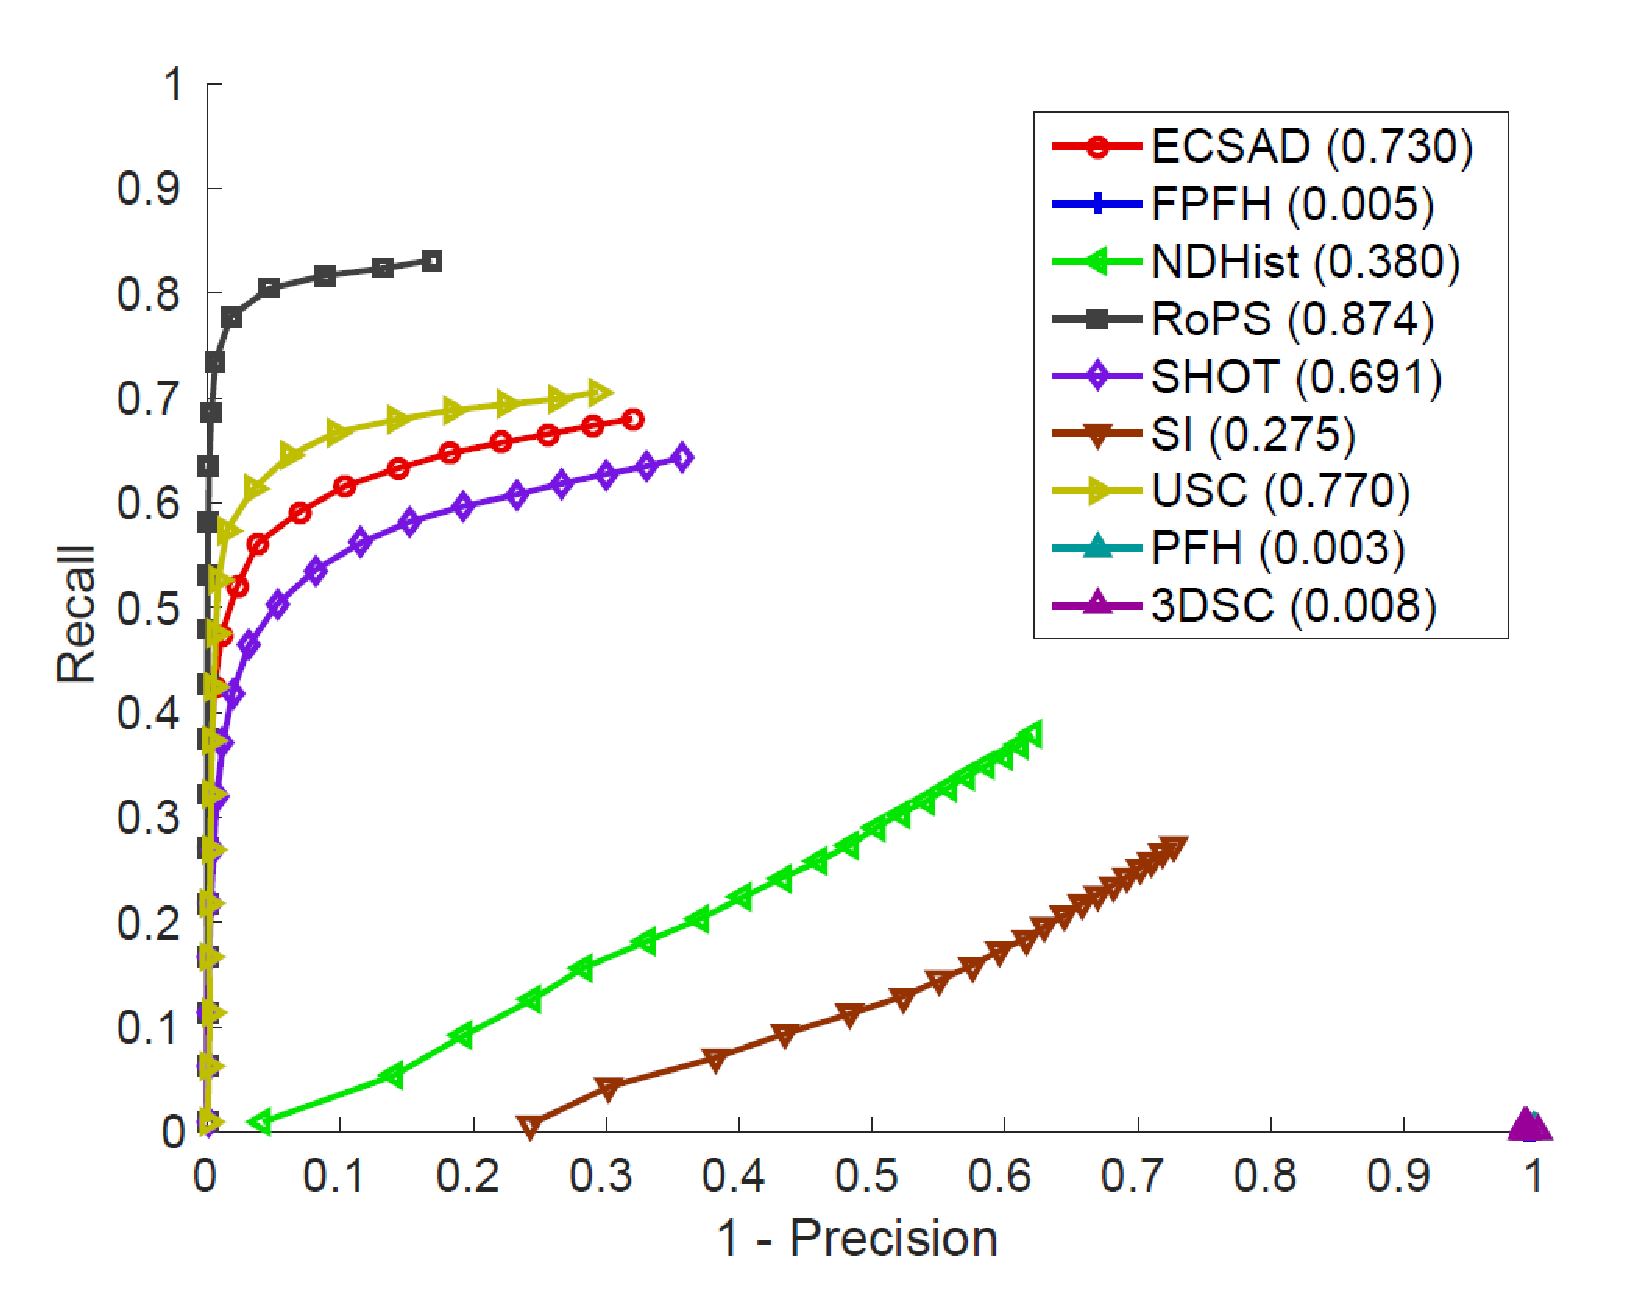
\includegraphics[width=1.0\linewidth, height= 0.7\linewidth, keepaspectratio]{img/PRC_1.pdf} 
\caption{Noise level 1 for STL dataset}\label{fig:stl_n1}
\end{minipage}\qquad
\begin{minipage}[b]{.3\textwidth}
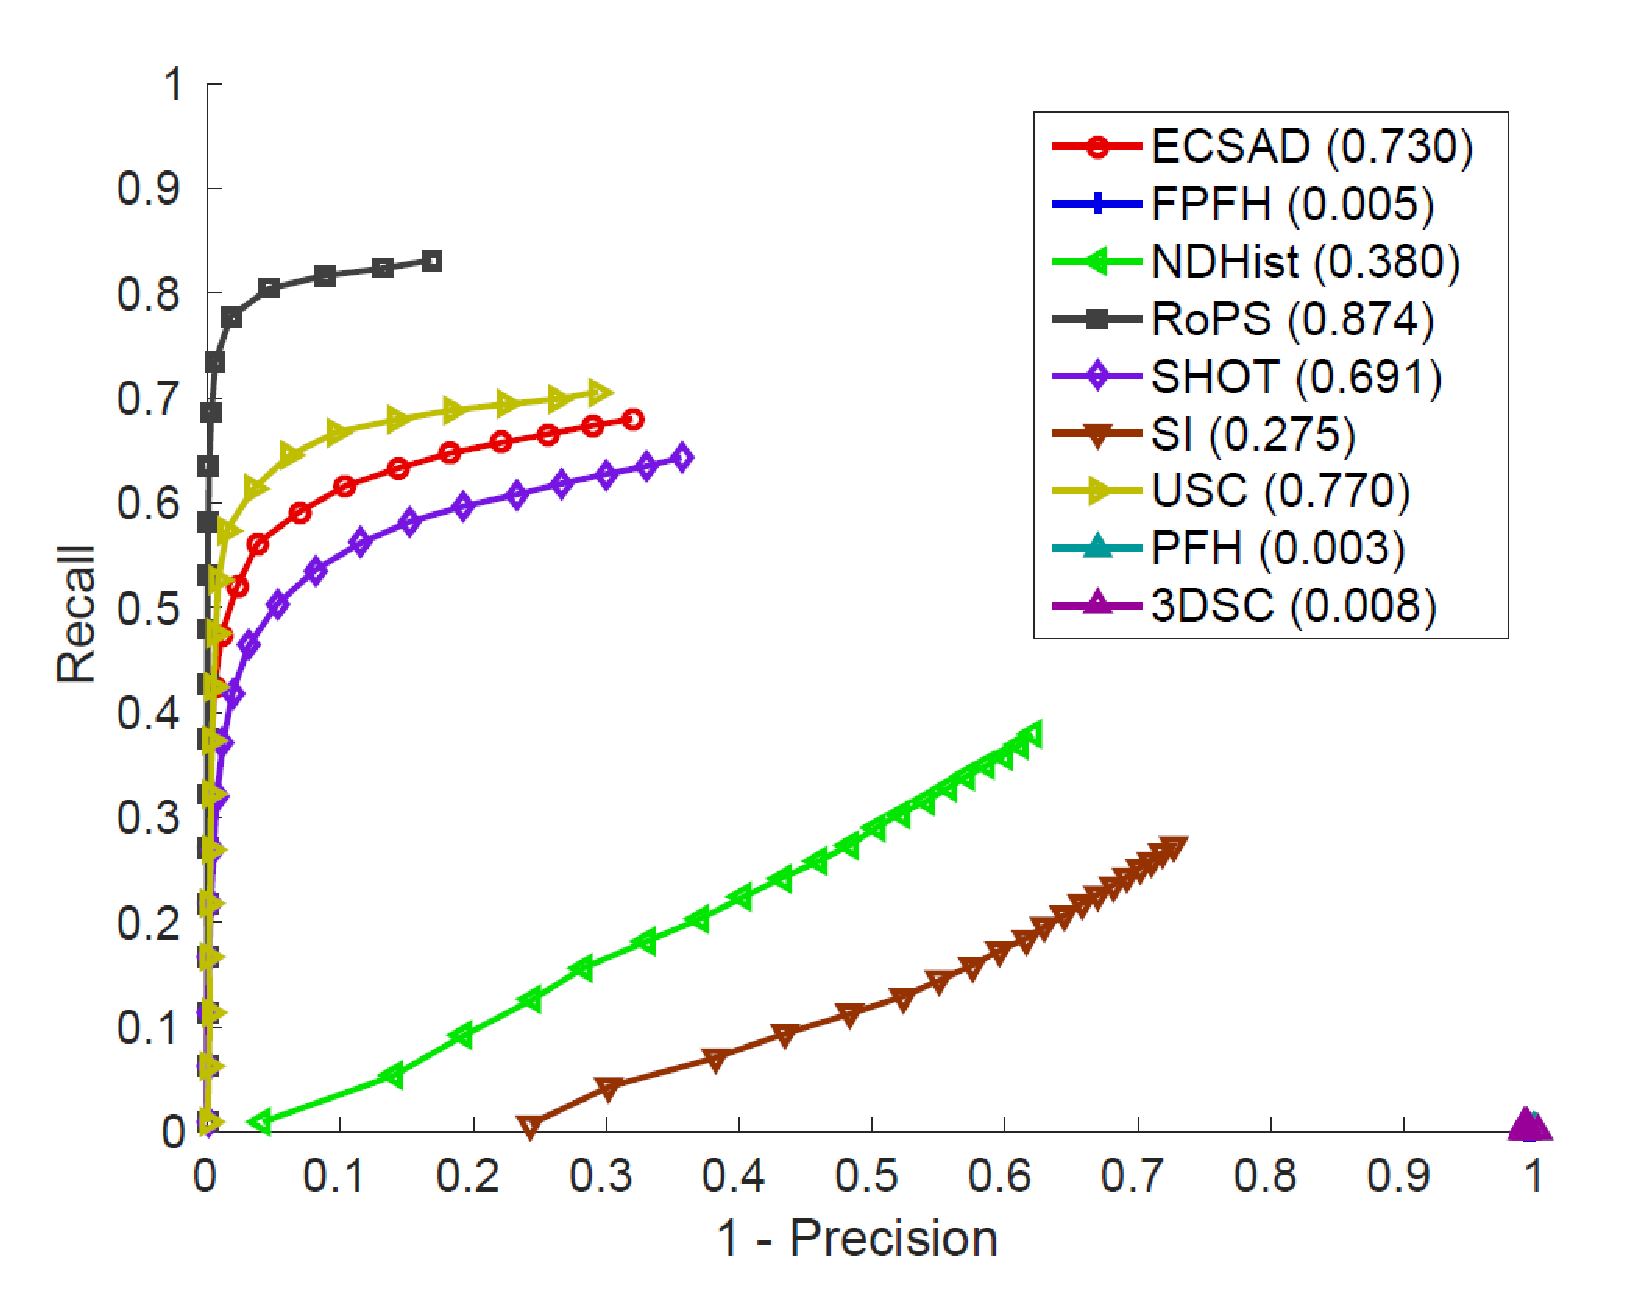
\includegraphics[width=1.0\linewidth, height= 1.0\linewidth, keepaspectratio]{img/PRC_1.pdf}
\caption{Noise level 2 for STL dataset}\label{fig:stl_n2}
\end{minipage}
\begin{minipage}[b]{.3\textwidth}
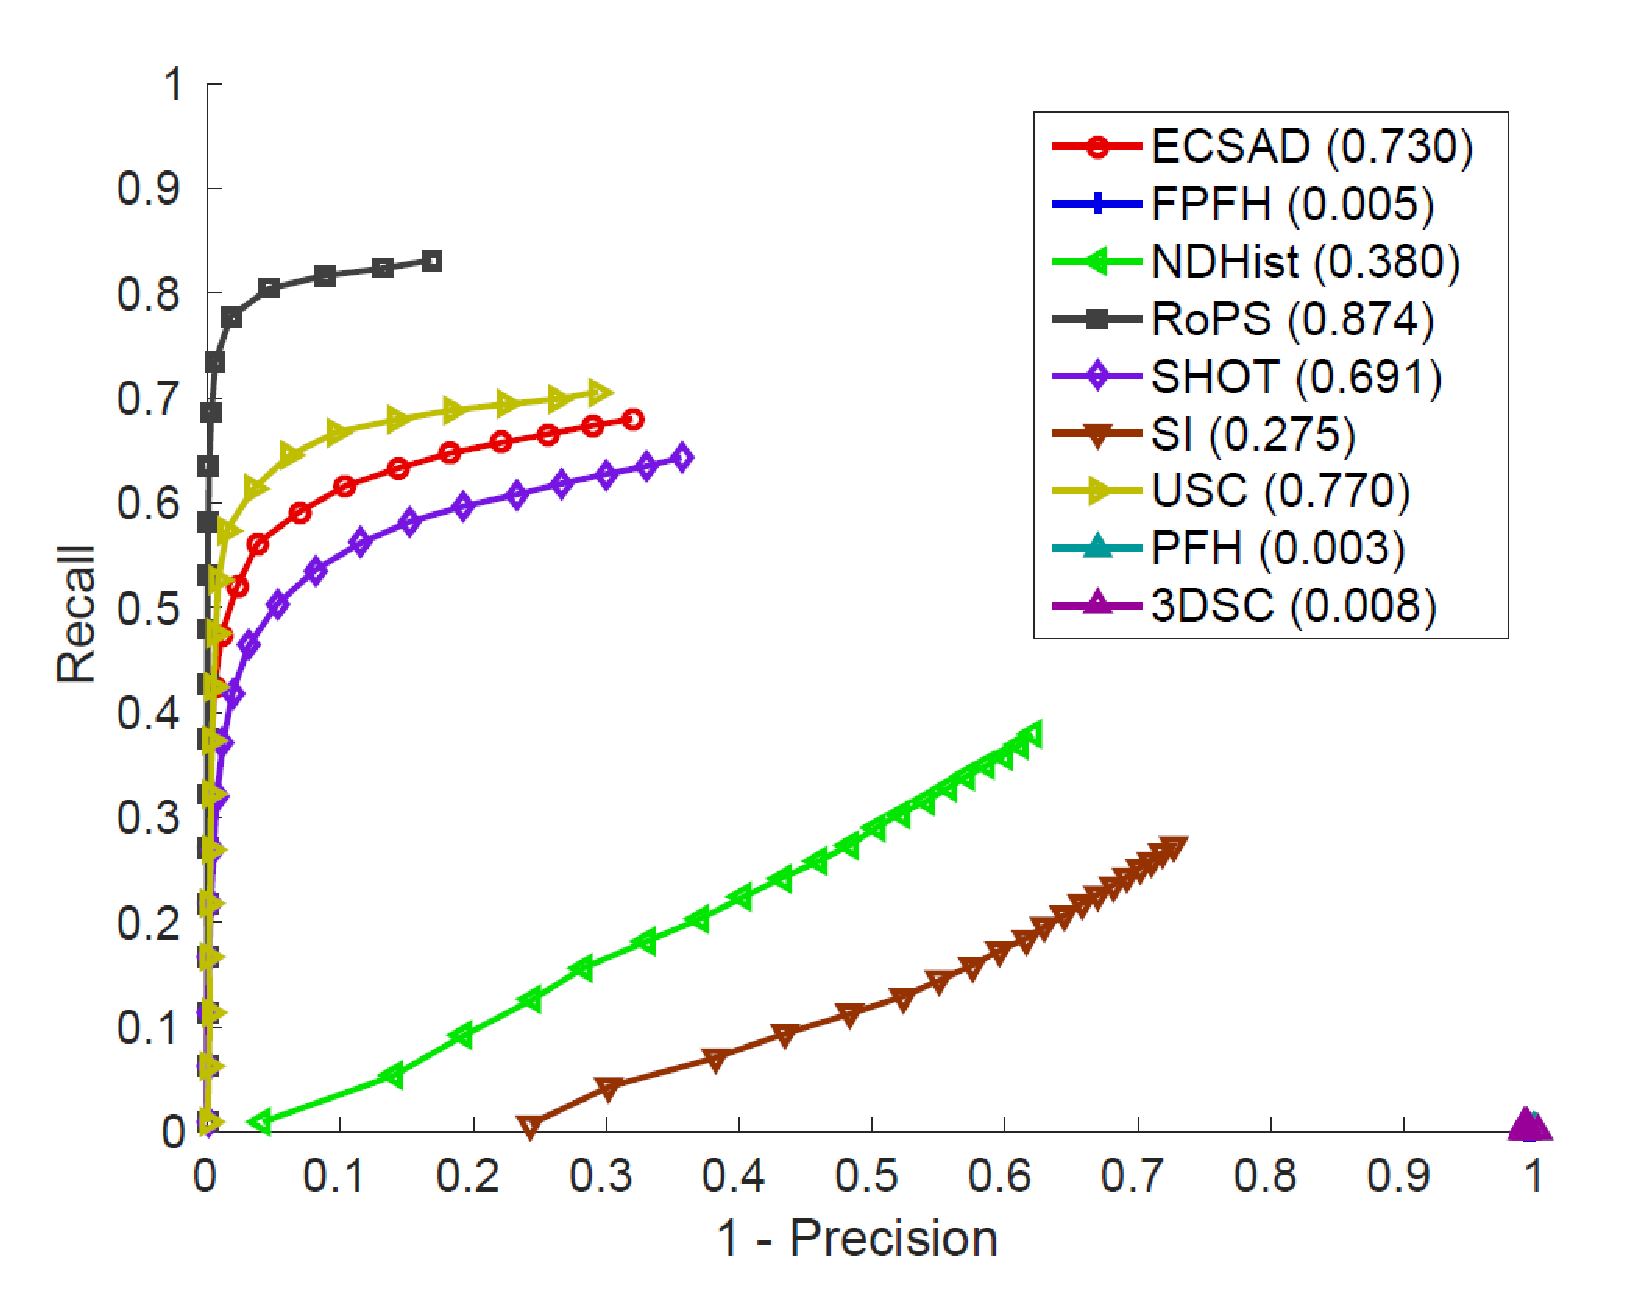
\includegraphics[width=1.0\linewidth, height= 1.0\linewidth, keepaspectratio]{img/PRC_1.pdf}
\caption{Noise level 3 for STL dataset}\label{fig:stl_n3}
\end{minipage}
\begin{minipage}[b]{.3\textwidth}
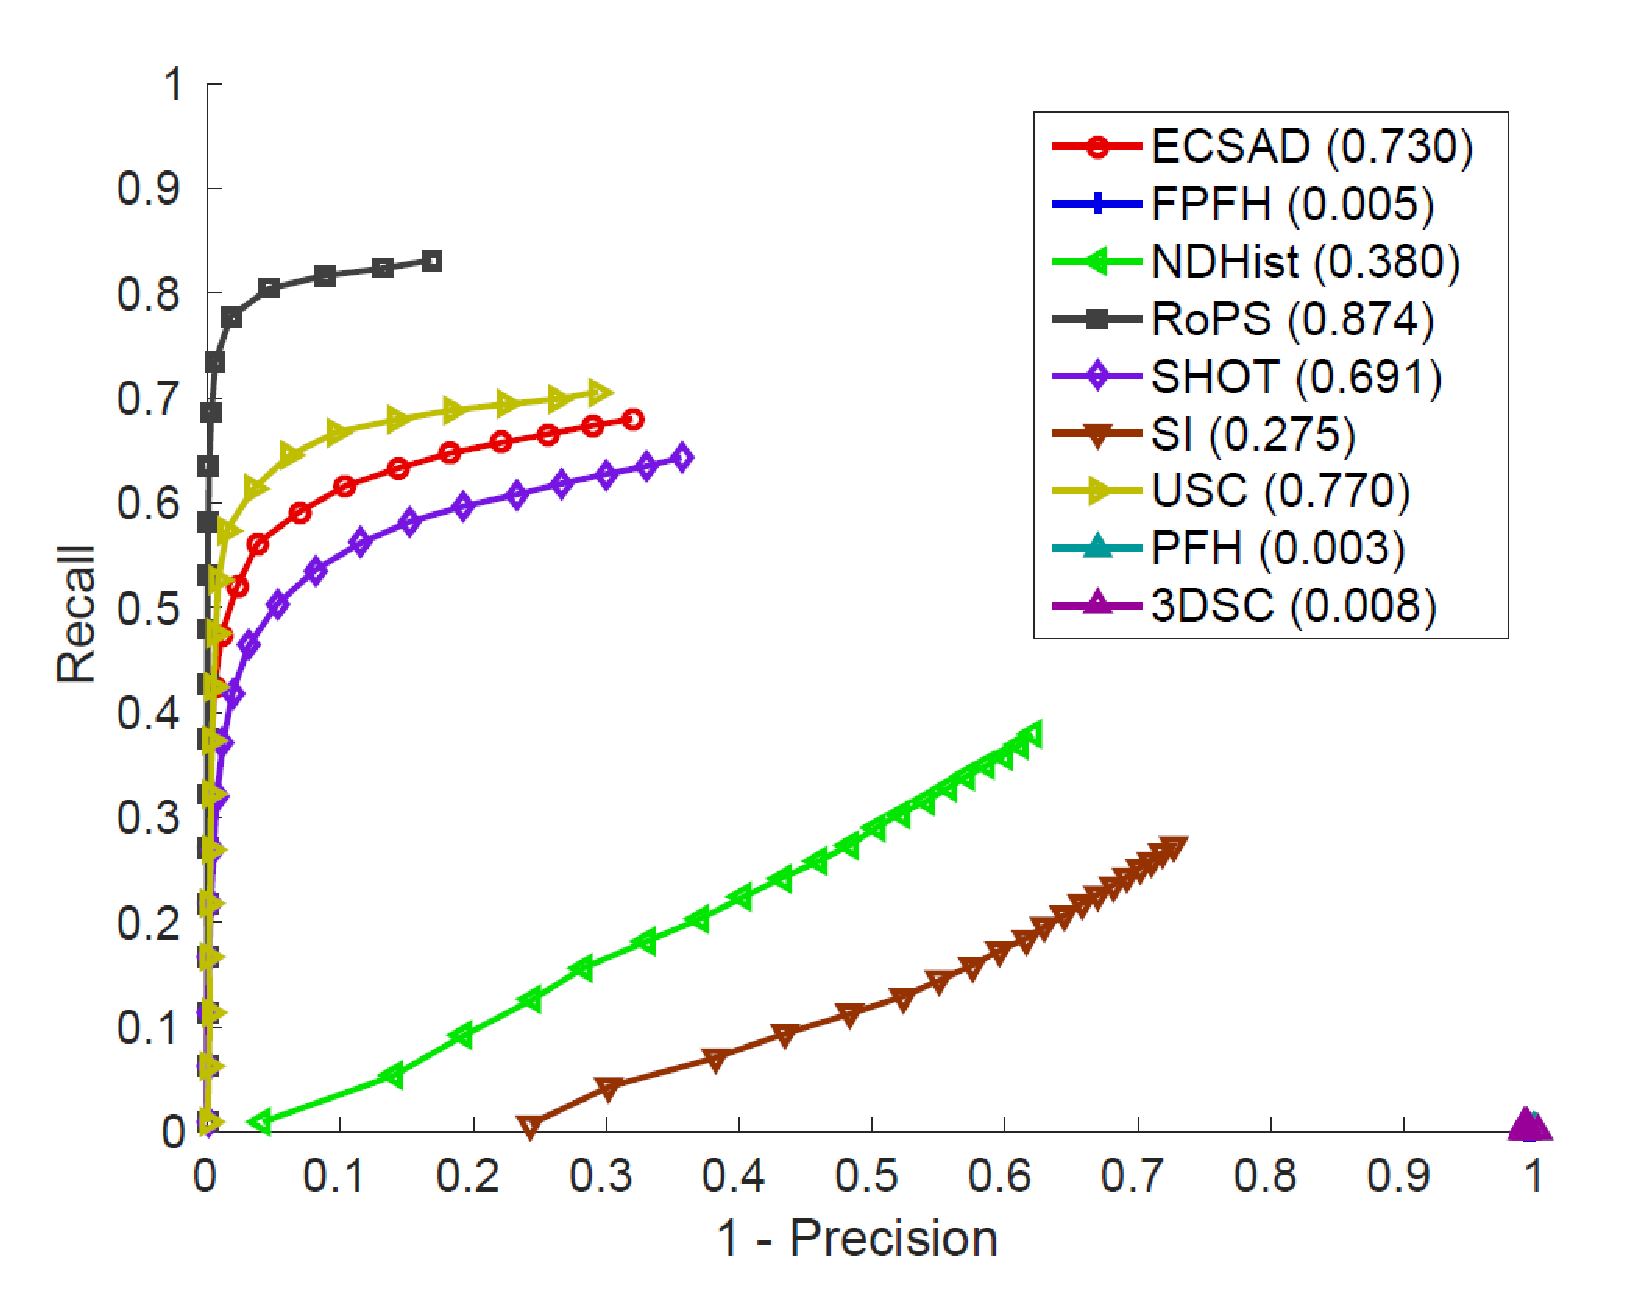
\includegraphics[width=1.0\linewidth, height= 1.0\linewidth, keepaspectratio]{img/PRC_1.pdf} 
\caption{Decimination level 1 for STL dataset}\label{fig:stl_d1}
\end{minipage}\qquad
\begin{minipage}[b]{.3\textwidth}
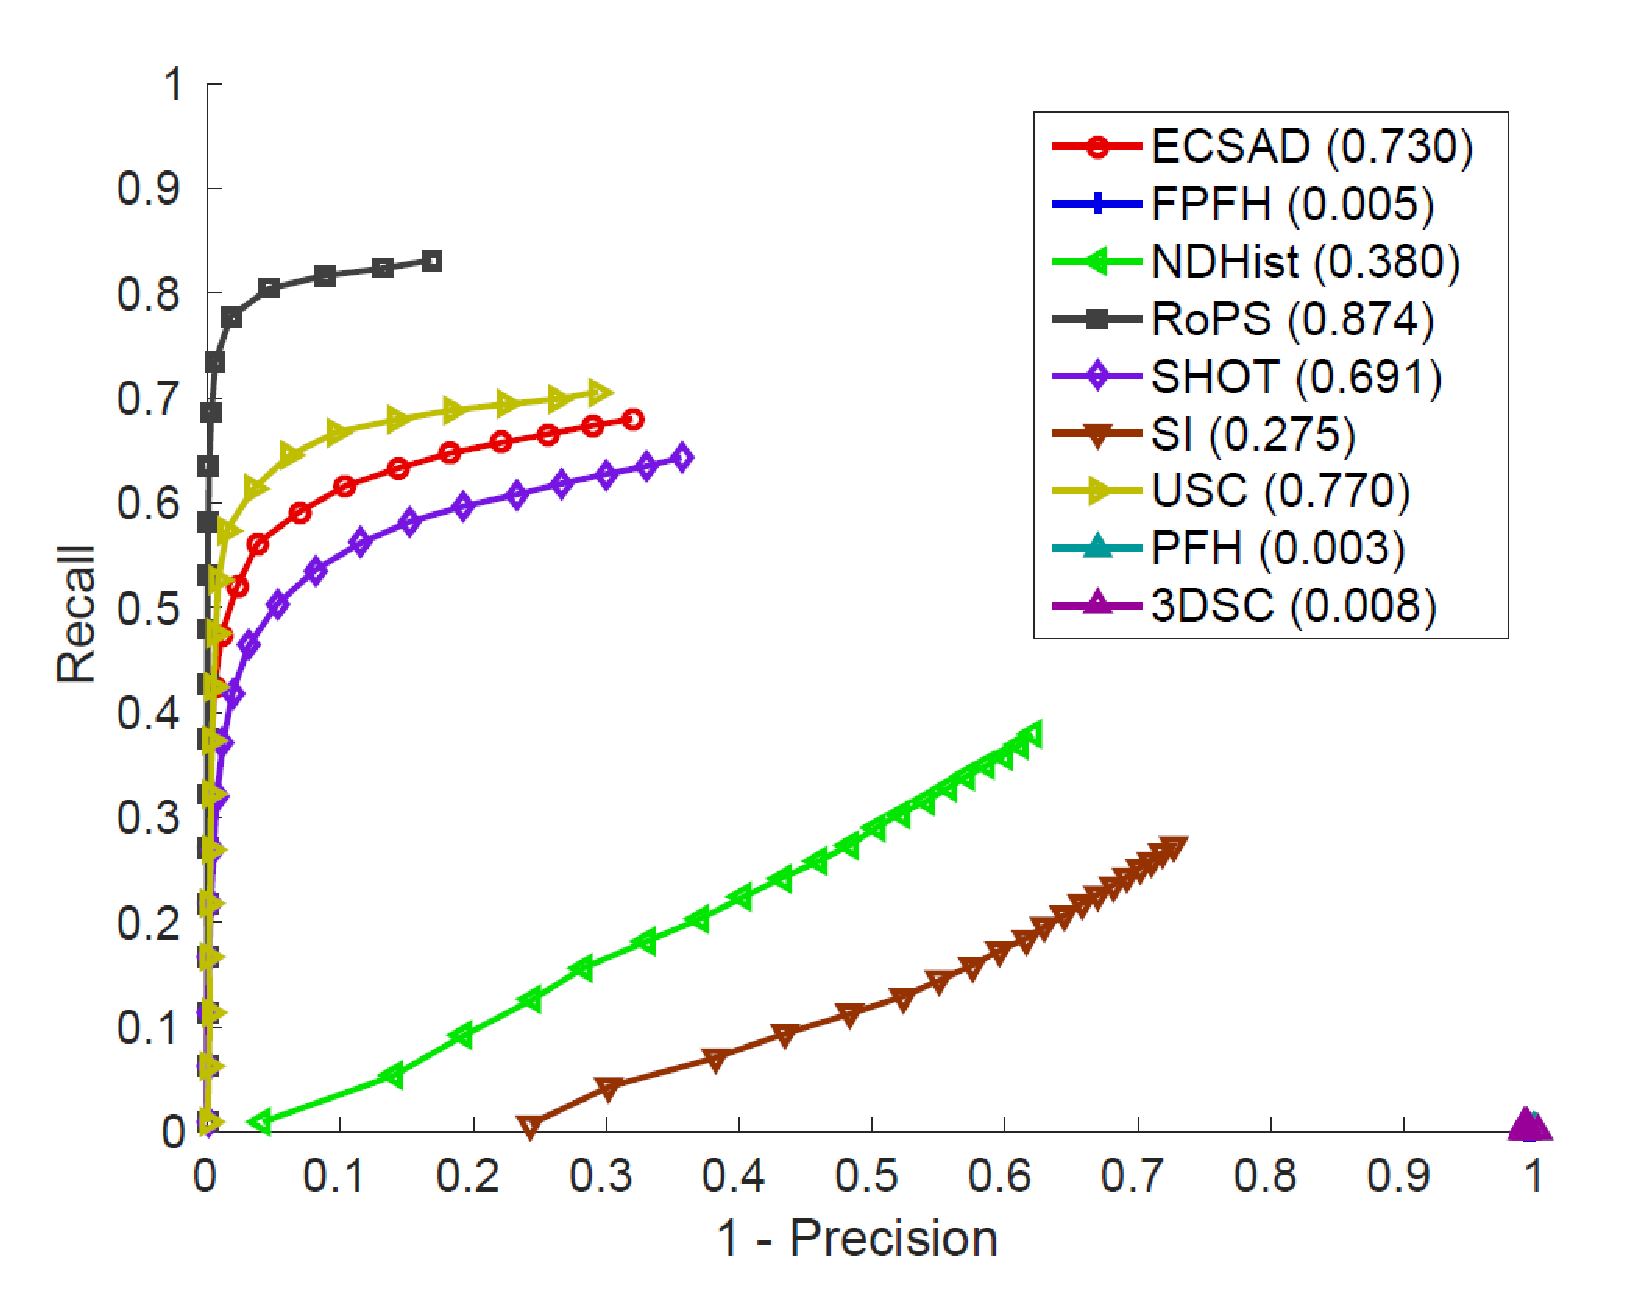
\includegraphics[width=1.0\linewidth, height= 1.0\linewidth, keepaspectratio]{img/PRC_1.pdf}
\caption{Decimination level 2 for STL dataset}\label{fig:stl_d2}
\end{minipage}
\begin{minipage}[b]{.3\textwidth}
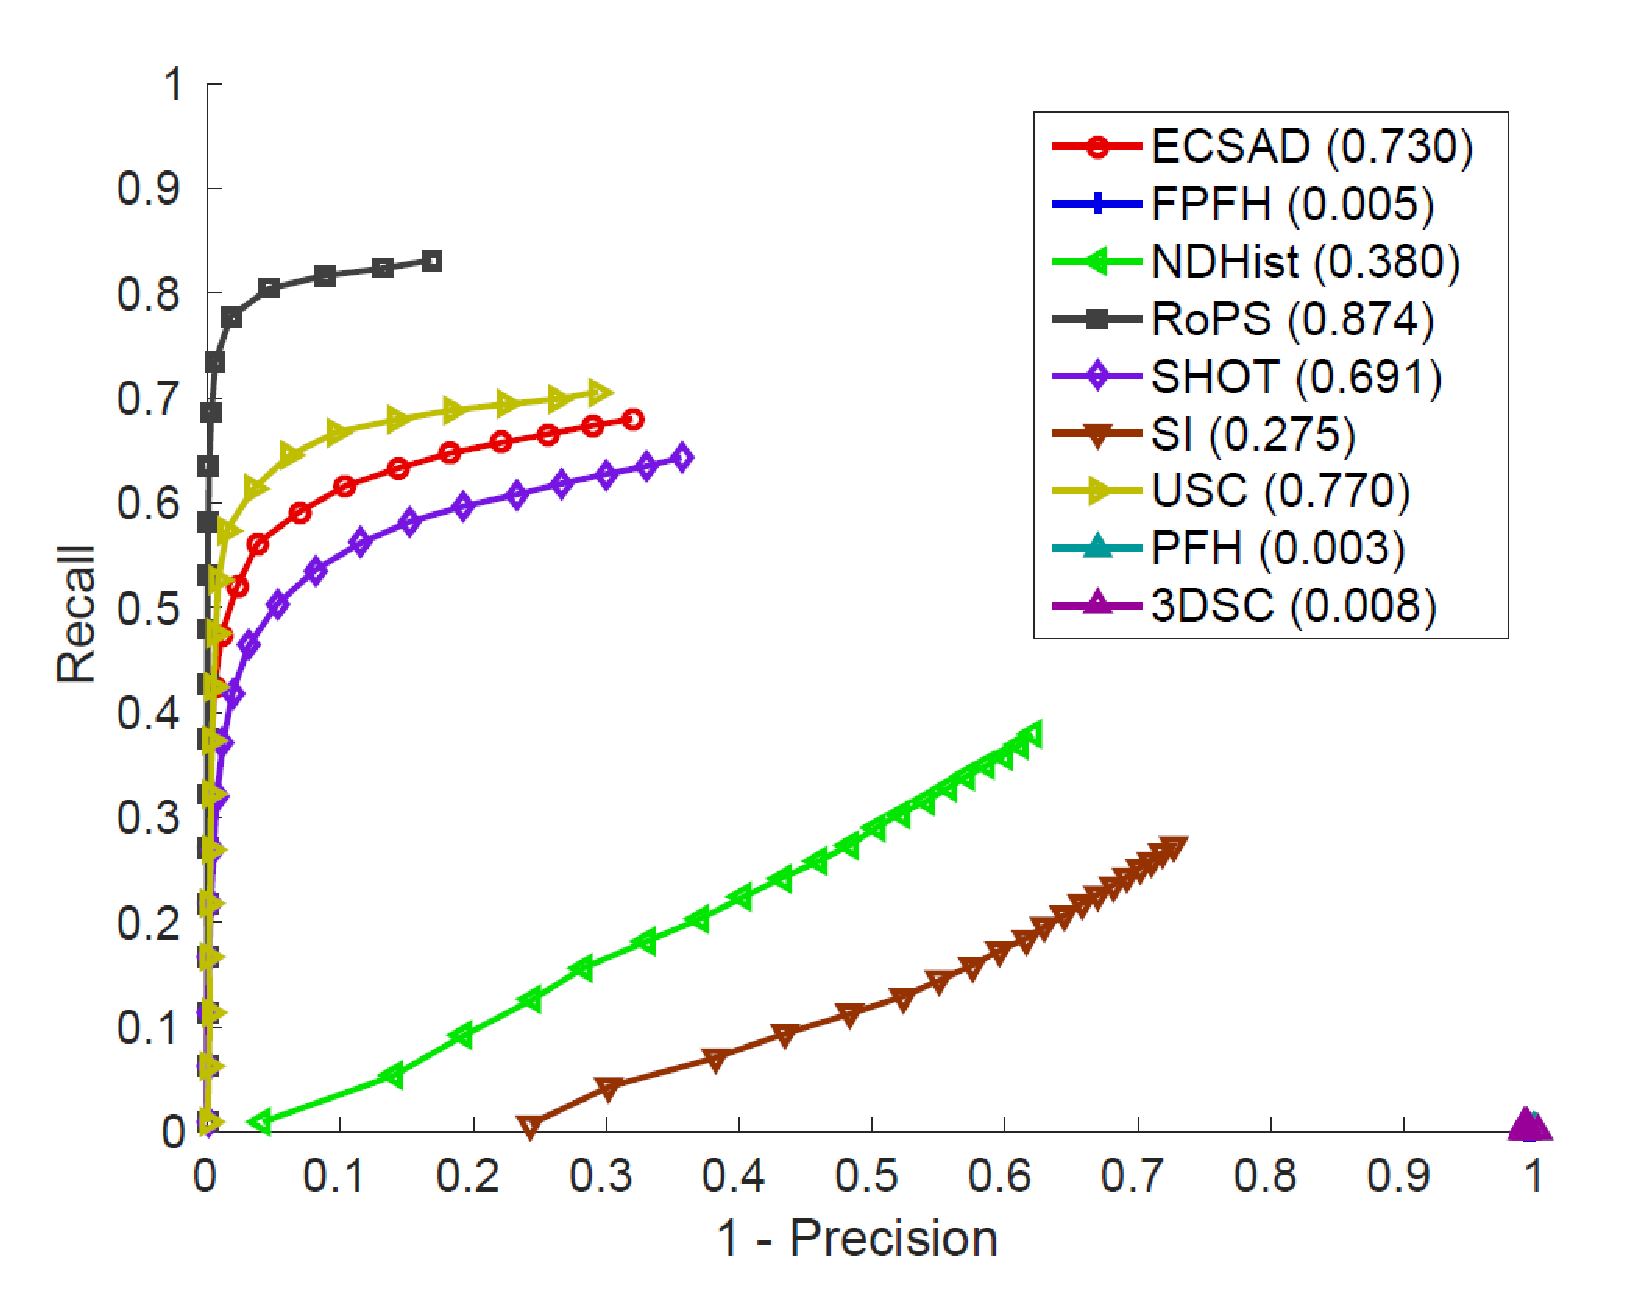
\includegraphics[width=1.0\linewidth, height= 1.0\linewidth, keepaspectratio]{img/PRC_1.pdf}
\caption{Decimination level 3 for STL dataset}\label{fig:stl_d3}
\end{minipage}
\end{figure*}


\begin{figure*}[htp]
\centering
\begin{minipage}[b]{.3\textwidth}
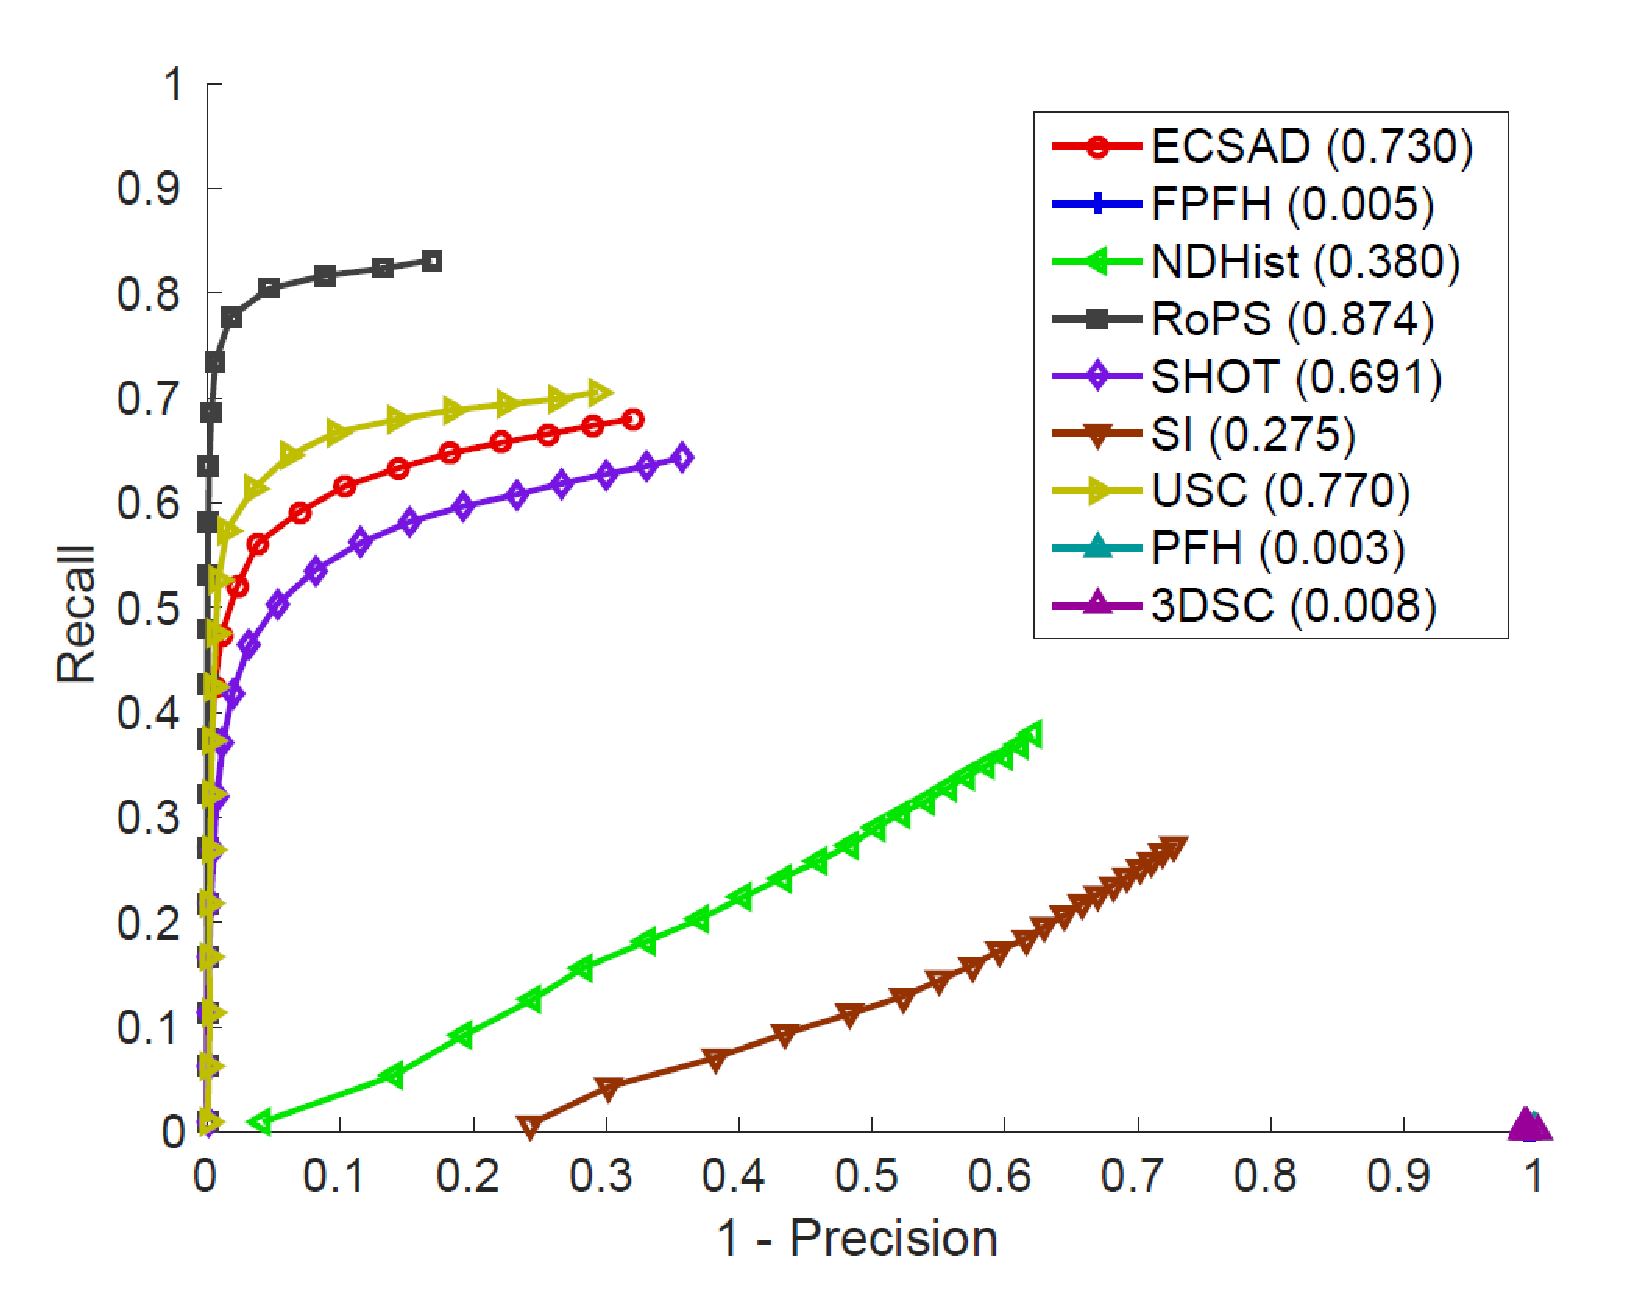
\includegraphics[width=1.0\linewidth, height= 1.0\linewidth, keepaspectratio]{img/PRC_1.pdf} 
\caption{Noise level 1 for Kinect dataset}\label{fig:kinect_n1}
\end{minipage}\qquad
\begin{minipage}[b]{.3\textwidth}
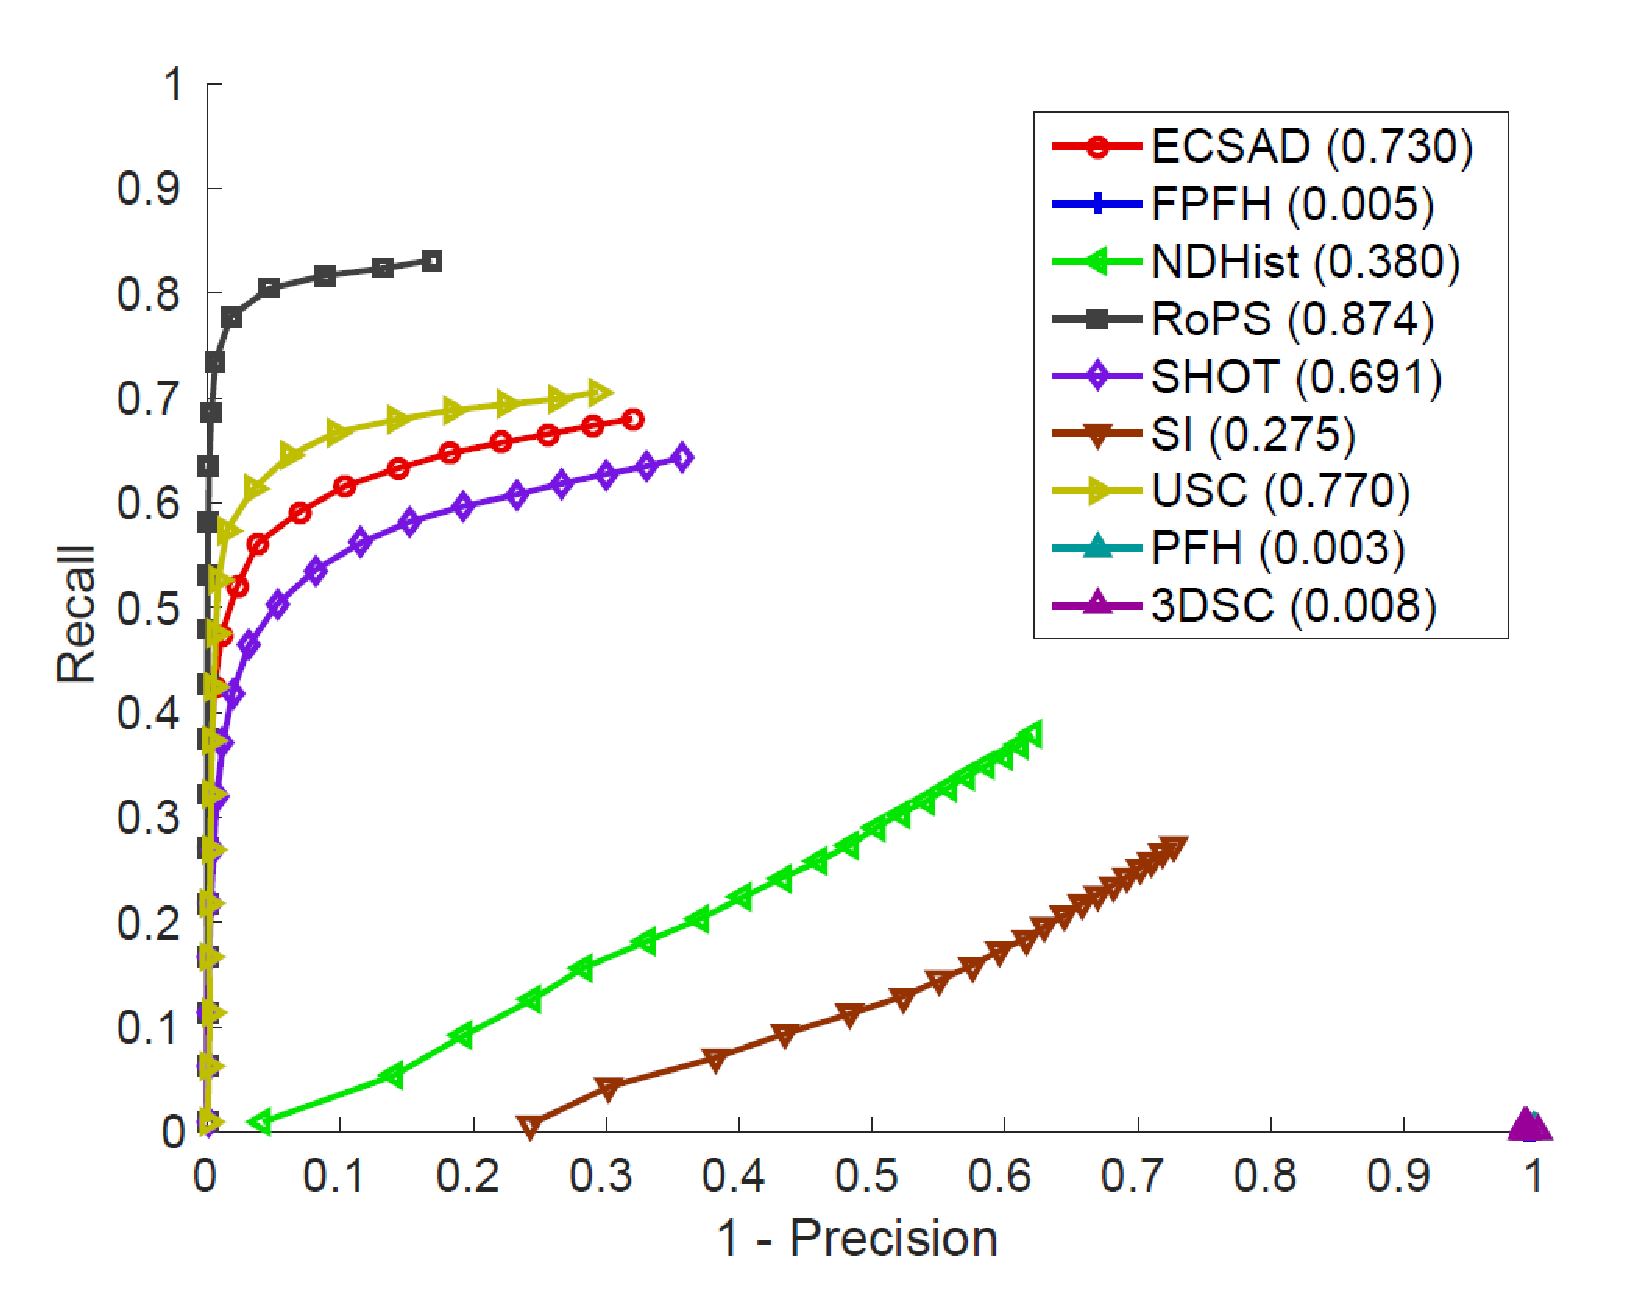
\includegraphics[width=1.0\linewidth, height= 1.0\linewidth, keepaspectratio]{img/PRC_1.pdf}
\caption{Noise level 2 for Kinect dataset}\label{fig:kinect_n2}
\end{minipage}
\begin{minipage}[b]{.3\textwidth}
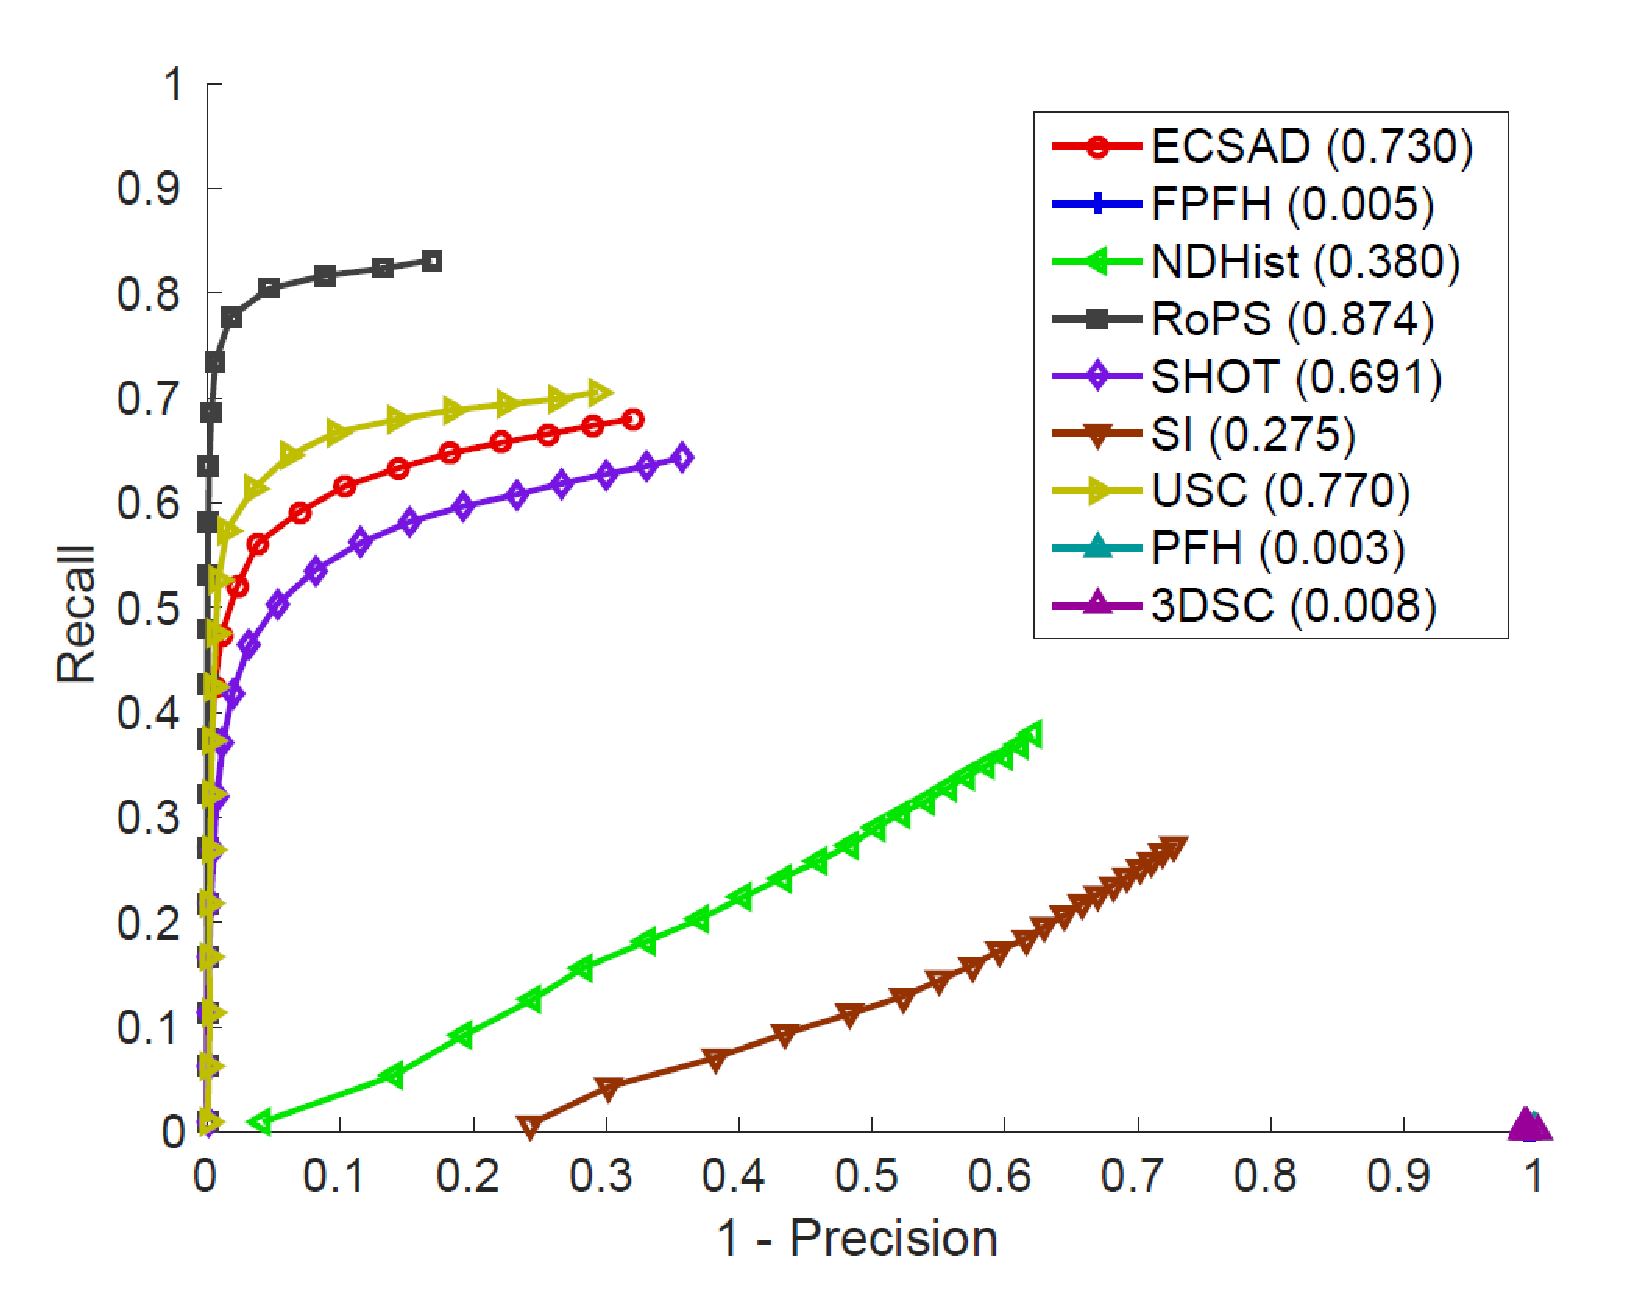
\includegraphics[width=1.0\linewidth, height= 1.0\linewidth, keepaspectratio]{img/PRC_1.pdf}
\caption{Noise level 3 for Kinect dataset}\label{fig:kinect_n3}
\end{minipage}
\begin{minipage}[b]{.3\textwidth}
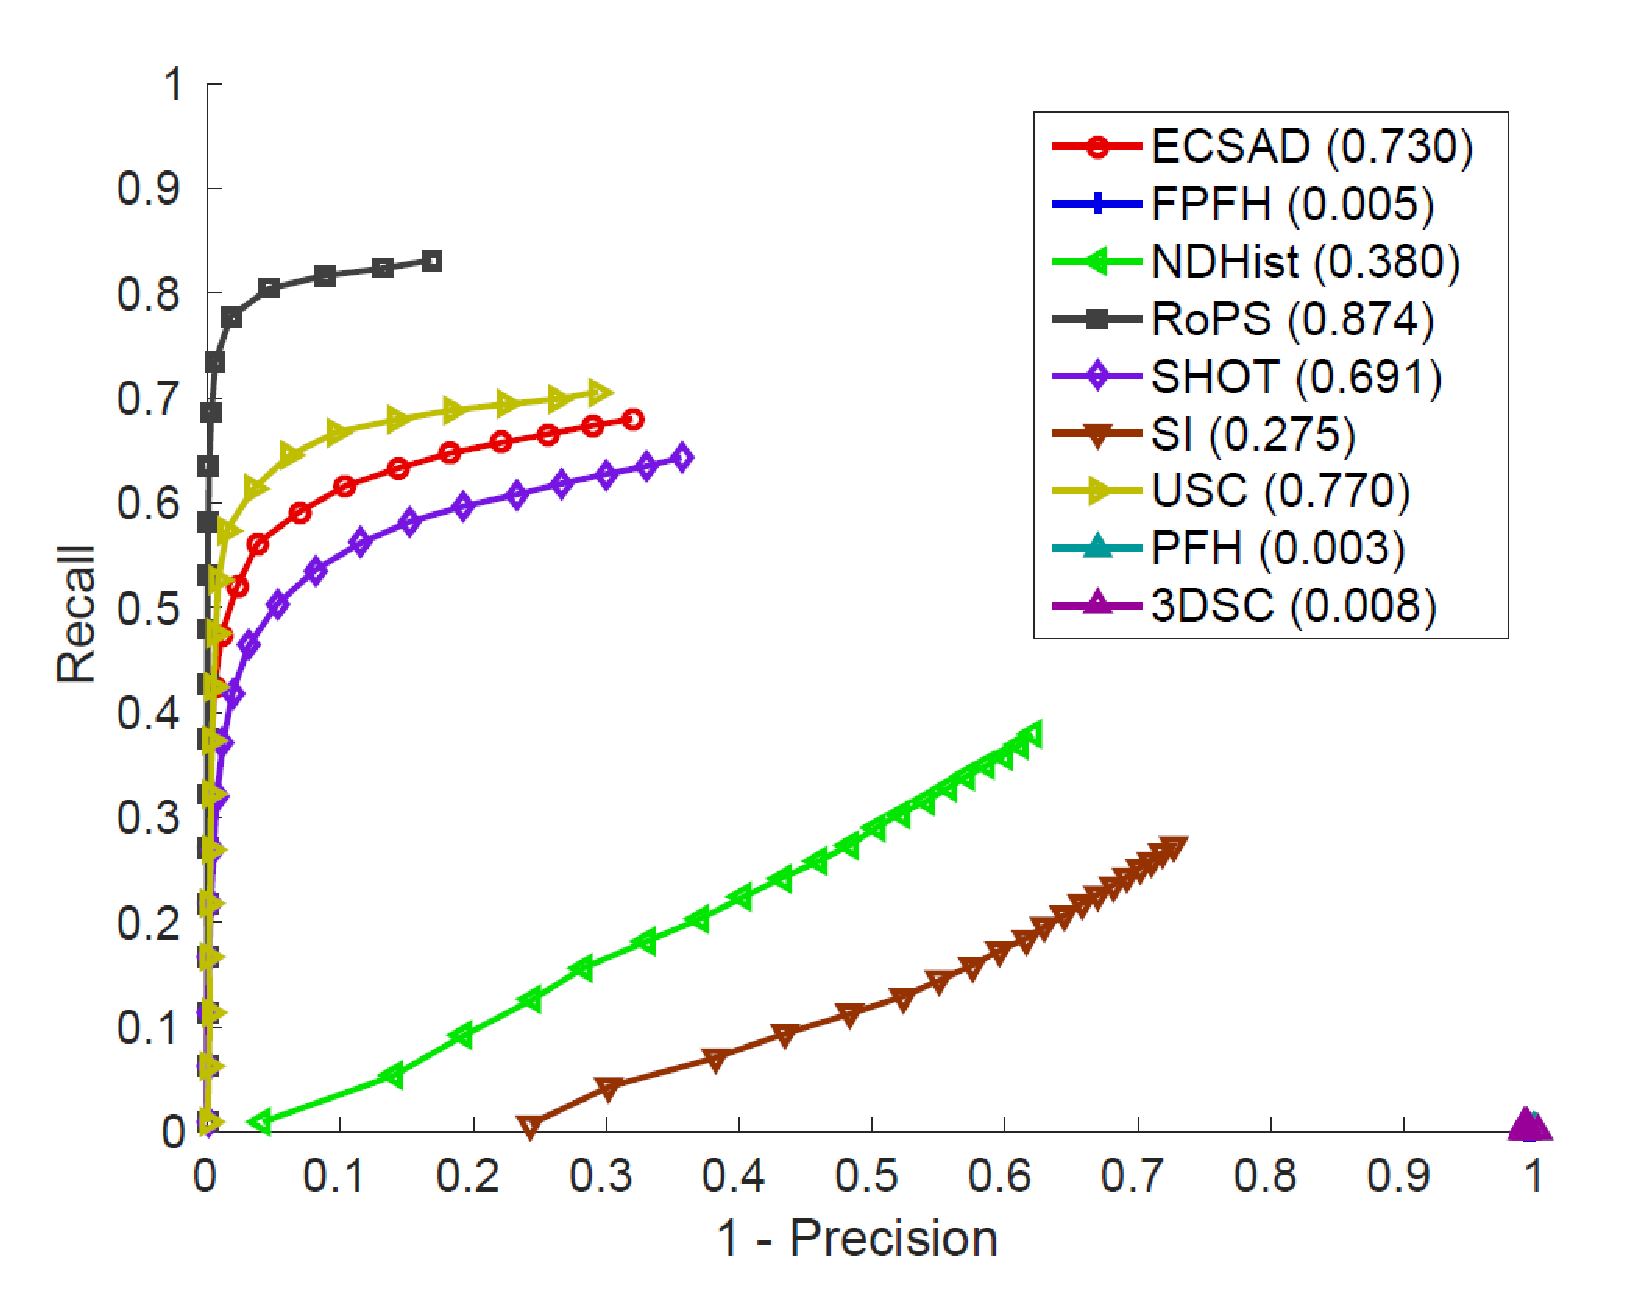
\includegraphics[width=1.0\linewidth, height= 1.0\linewidth, keepaspectratio]{img/PRC_1.pdf} 
\caption{Decimination level 1 for Kinect dataset}\label{fig:kinect_d1}
\end{minipage}\qquad
\begin{minipage}[b]{.3\textwidth}
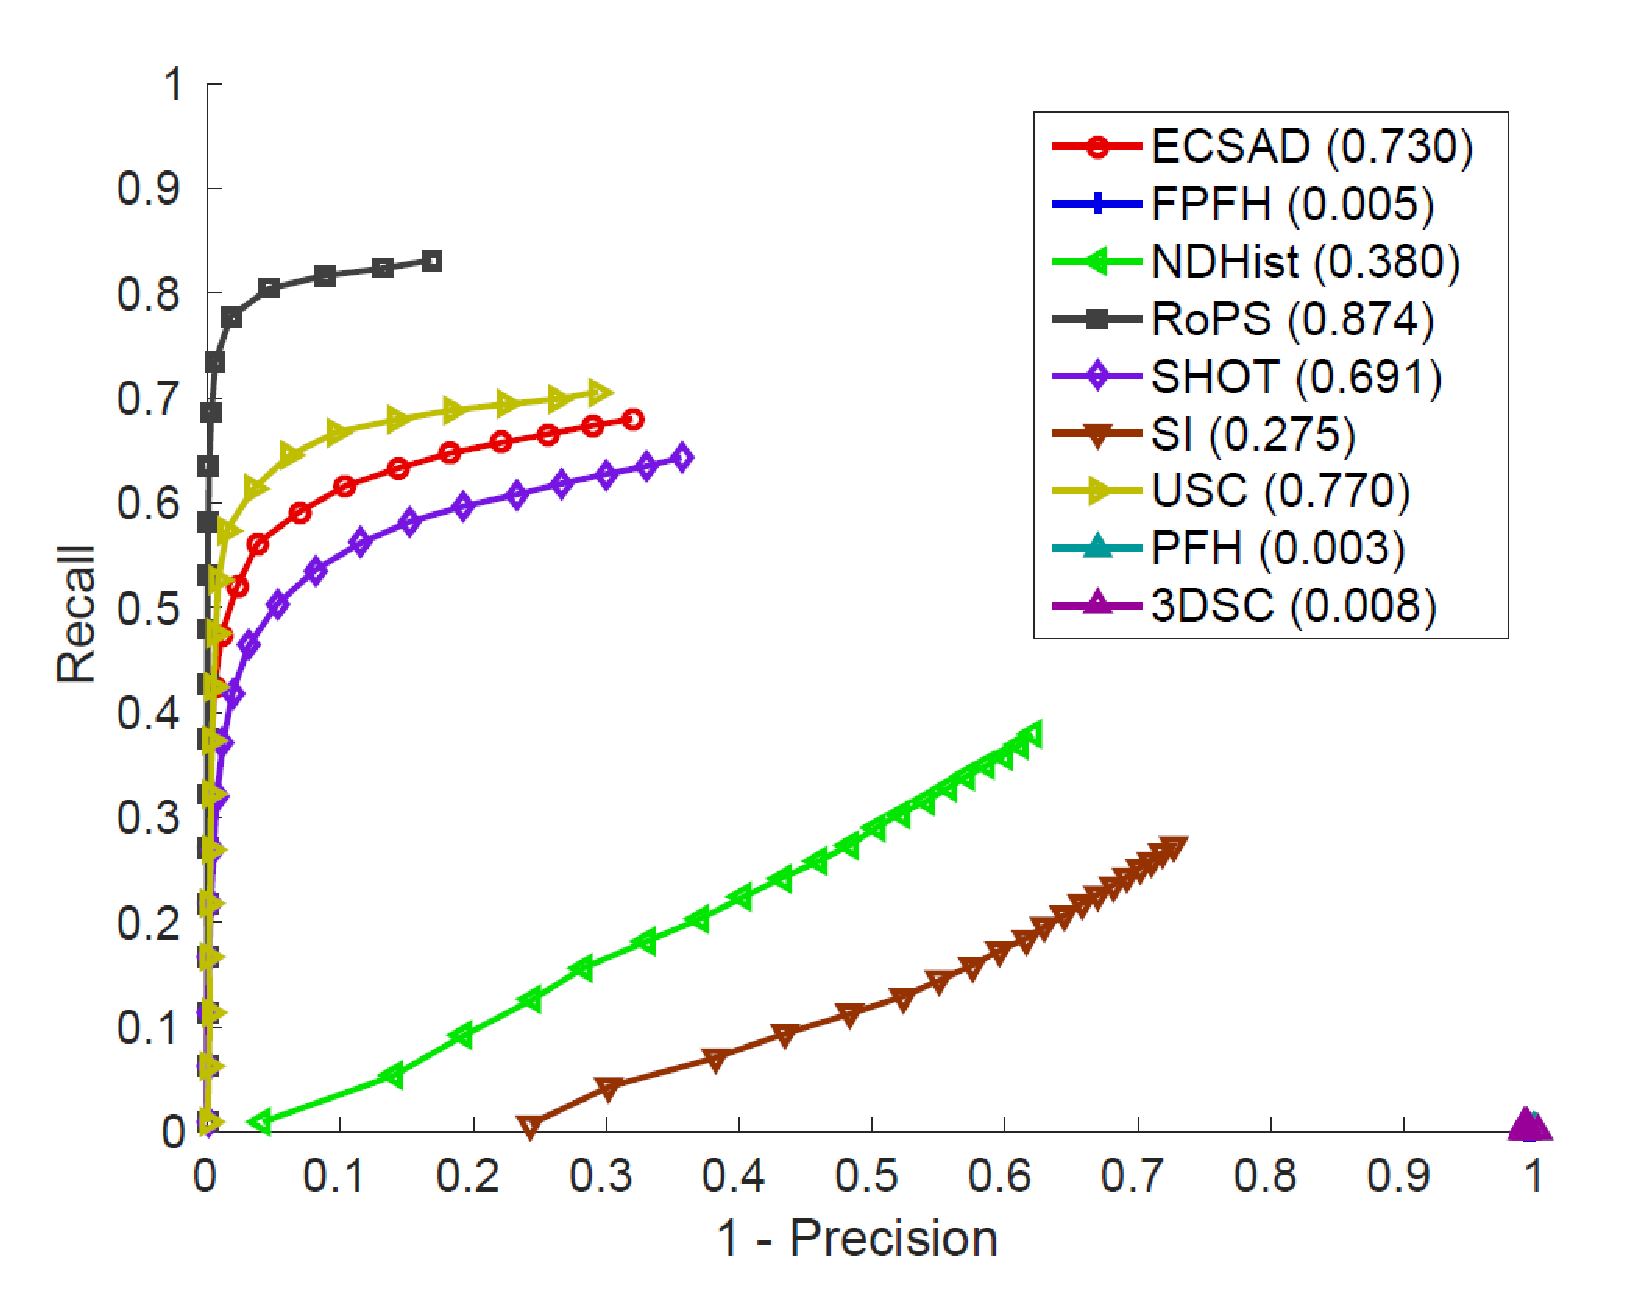
\includegraphics[width=1.0\linewidth, height= 1.0\linewidth, keepaspectratio]{img/PRC_1.pdf}
\caption{Decimination level 2 for Kinect dataset}\label{fig:kinect_d2}
\end{minipage}
\begin{minipage}[b]{.3\textwidth}
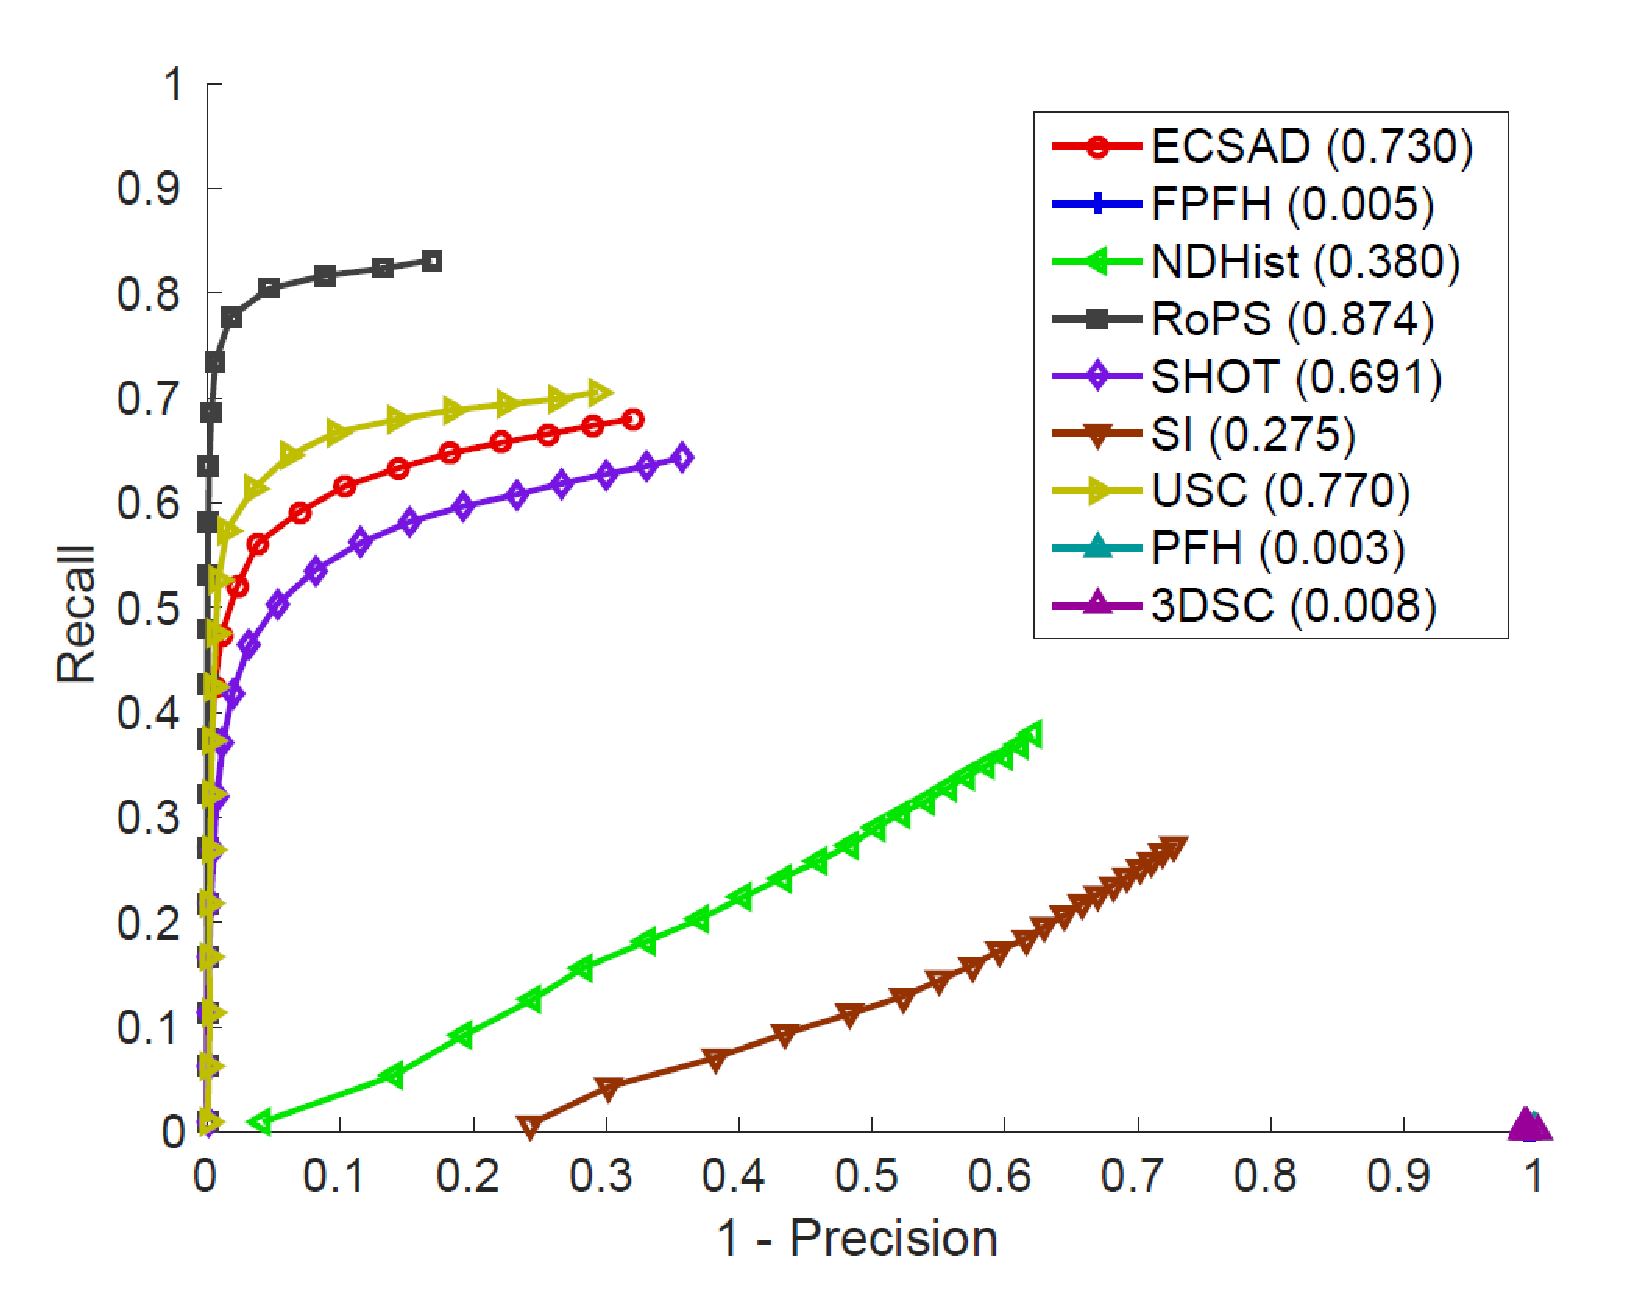
\includegraphics[width=1.0\linewidth, height= 1.0\linewidth, keepaspectratio]{img/PRC_1.pdf}
\caption{Decimination level 3 for Kinect dataset}\label{fig:kinect_d3}
\end{minipage}
\end{figure*}


\begin{table}[ht]
\centering
\begin{tabular}{llllll}
\hline
\textbf{Feature} & \textbf{STL} & \textbf{Kinect} & \textbf{Gr. 1}  &\textbf{Gr. 2} &\textbf{Gr. 3} \\
\hline
 \textbf{\textit{ECSAD}}  & 0.00 & 0.00 & 0.00 & 0.00 & 0.00 \\
 \textbf{\textit{FPFH}}   & 0.00 & 0.00 & 0.00 & 0.00 & 0.00 \\
 \textbf{\textit{NDHIST}} & 0.00 & 0.00 & 0.00 & 0.00 & 0.00 \\
 \textbf{\textit{ROPS}}   & 0.00 & 0.00 & 0.00 & 0.00 & 0.00 \\
 \textbf{\textit{SHOT}}   & 0.00 & 0.00 & 0.00 & 0.00 & 0.00 \\
 \textbf{\textit{SI}}     & 0.00 & 0.00 & 0.00 & 0.00 & 0.00 \\
 \textbf{\textit{USC}}    & 0.00 & 0.00 & 0.00 & 0.00 & 0.00 \\
 \textbf{\textit{PFH}}    & 0.00 & 0.00 & 0.00 & 0.00 & 0.00 \\
 \textbf{\textit{3DSC}}   & 0.00 & 0.00 & 0.00 & 0.00 & 0.00 \\
 \hline
 \hline
 \textbf{\textit{Mean ($\lambda$)}}   & 0.00 & 0.00 & 0.00 & 0.00 & 0.00 \\
 \hline
 \\
\end{tabular}
\caption{Overall recognition rates. \textbf{First column:} Features descriptors. \textbf{Second column:} Recognition rate for the full stl dataset. \textbf{Third column:} Recognition rate for the full kinect dataset. \textbf{Fourth column:} Recognition rate for group 1 object subset. \textbf{Fifth column:} Recognition rate for group 2 object subset. \textbf{Sixth column:} Recognition rate for group 2 object subset.}
\label{tab:recognition}
\end{table}

%-------------------------------------------------------------------------
\section{Discussion \& Conclusion}\label{sec:conclusion}

%-------------------------------------------------------------------------


{\small
\bibliographystyle{3dv2016authorkit/latex/ieee}
\bibliography{bib}
}

\end{document}
